% !TEX root = ../../book.tex
%\hfill
%\par\vspace{\baselineskip}

\chapter{Modeling Trade Data}

\section{Normalizing Analytics}
One of the challenging aspects of execution unlike other algorithmic trading subject is the large number of different types of stocks such strategies have to apply to. The same strategy will need to work for super liquid instruments that trade like water at the minimum tick size, and illiquid stocks that trade only very infrequently at wide spreads; Stock that have very stable and large sizes at the inside market, and stocks whose nbbo changes many times every second. To complicate matters further the market micro-structure of each stock is not constant throughout the day and certain days (sometime called "Special Days" ) stock behavior is often very different. These changes are to a large extent predictable and execution strategies are expected to adapt to them. 
\newline
\par
Intraday variations are well documented and are rooted in institutional investor behavior. Immediately after the open there is a lot of trading activity as investor incorporate the effect of overnight news. The increased uncertainty on the stock valuation is reflected by a much higher volatility and spread. Once the period of so called Price Discovery is over (usually within 15-30m in US markets), the trading behavior settles in and activity is reduced and so do spreads and volatility. Activity resumes towards the end of the day in particular due to the  fact that many funds are marked to the day's closing price. European markets have further predictable "bumps" in and around the US market open as the markets absorbs the reaction of US investors.
\newline
\par
One important source of inter-day variabilty is the impact of "Special Days" such as futures, and options expiration, earning announcements, Fed announcements, etc. On such occasions the activity patterns are systematically different. For  example the trading activity during futures/options expiration is heavily tilted towards the close since the settlement prices are related to the closing price on that day. On Fed announcement days trading activity slows to a trick ahead of the announcement as investor await any surprise decision. Activity jumps immediately after to incorporate any relevant information.

The complexity of dealing in a systematic way all the above variability is  daunting. One could (and in some cases arguably should) apply different approaches to achieve the same benchmark for different types of stocks and different days or time of day but that is never done in practice as it would be completely unwieldy and prohibitively expensive to build and maintain. What is one to do?

The common practitioner's approach is to parametrize many of the trading decisions using normalizing features, variables that help adapt the decision to a particular situation. 

This section provides a high level review of the most common analytics and gives pointers to modeling approaches commonly used to tackle them.  This subject is quite broad an, while extremely important in practice, has gotten very limited treatment in academic research something we feel should be rectified. In this section, while likely not scientifically satisfying, we  will thus only provide a relatively coarse treatment of the subject from a practitioner perspective. It should however be sufficient as a starting point for anybody attempting to build basic Execution Algorithms and will provide a foundation for deepening the subject.

\subsection{Basic Analytics}
\subsubsection{Order Size Normalization: ADV}
A trader needs to execute an order for 1M shares of XYZ. Is this a big order she will have to carefully manage or a tiny order she can simply "fire and forget".  Intuitively, from the trading perspective, due to  the large difference in stock characteristics and liquidity, order size should be viewed as a relative measure. The most commonly used order size normalizer used by practitioners is the ADV (Average Daily Volume). While the term Average Daily Volume has a specific mathematical meaning it is more often than not used as a generic term for a volume location measure.  Even for something seemingly so mundane a topic (ADV is actually very important for order sizing, position limits, etc) there are important considerations and decisions to make: What location measure to use? Average, Median, some other measure robust to outliers? Over what horizon? How to treat special days? The answer is likely application specific and there is very little consensus or rigorous study of the impact of using different measures.
 	
	\begin{figure}[!ht]
		\centering
			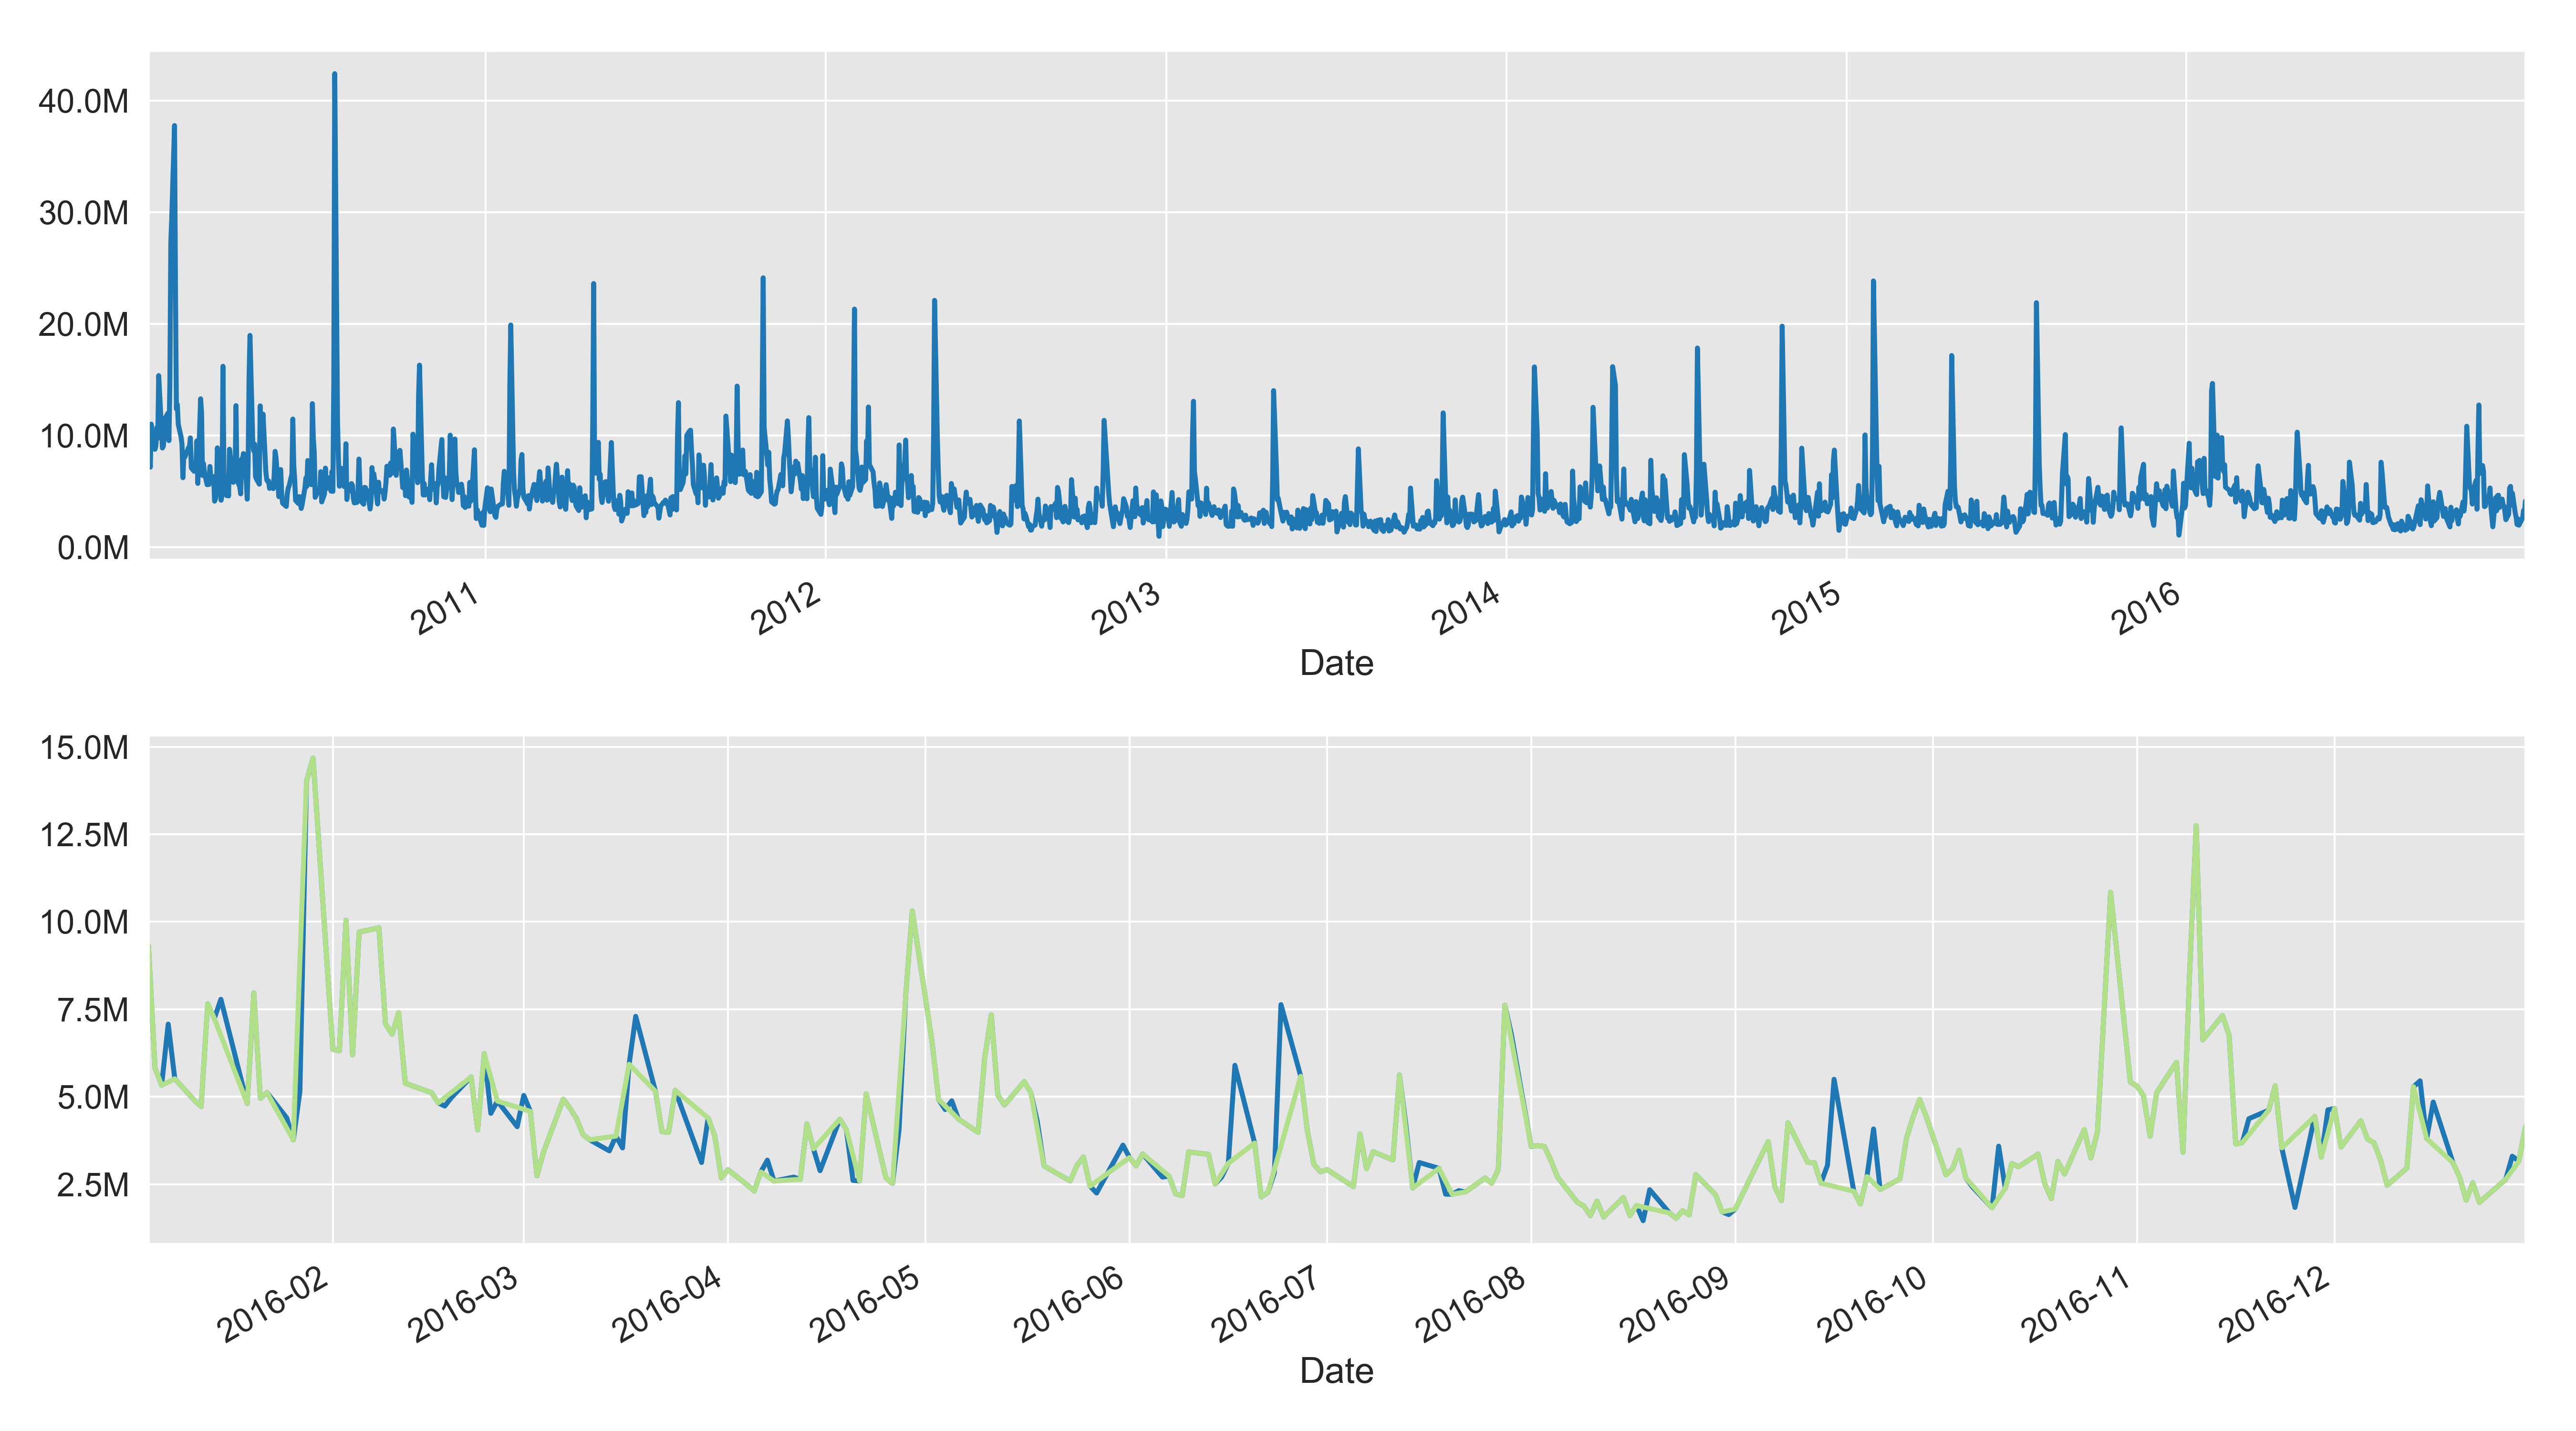
\includegraphics[width=0.75\textwidth]{chapters/chapter_trade_data_models/figures/daily_volume.png} 
		\caption{Daily Volume.Notice how volatile the data is. Strongly autocorrelated with periodic predictable spikes for special days and unpredictable 'surprises' \label{fig:daily_volume}}
	\end{figure}
	
As a baseline metric that 64 days Mean or Median daily volume are probably the most commonly used metric in the investment community. The reason behind it is that 64 days horizon reflects length of a quarterly earning cycle and thus it's viewed as incorporating  all the seasonal effects of the daily volume. See 
	
	\begin{figure}[!ht]
		\centering
			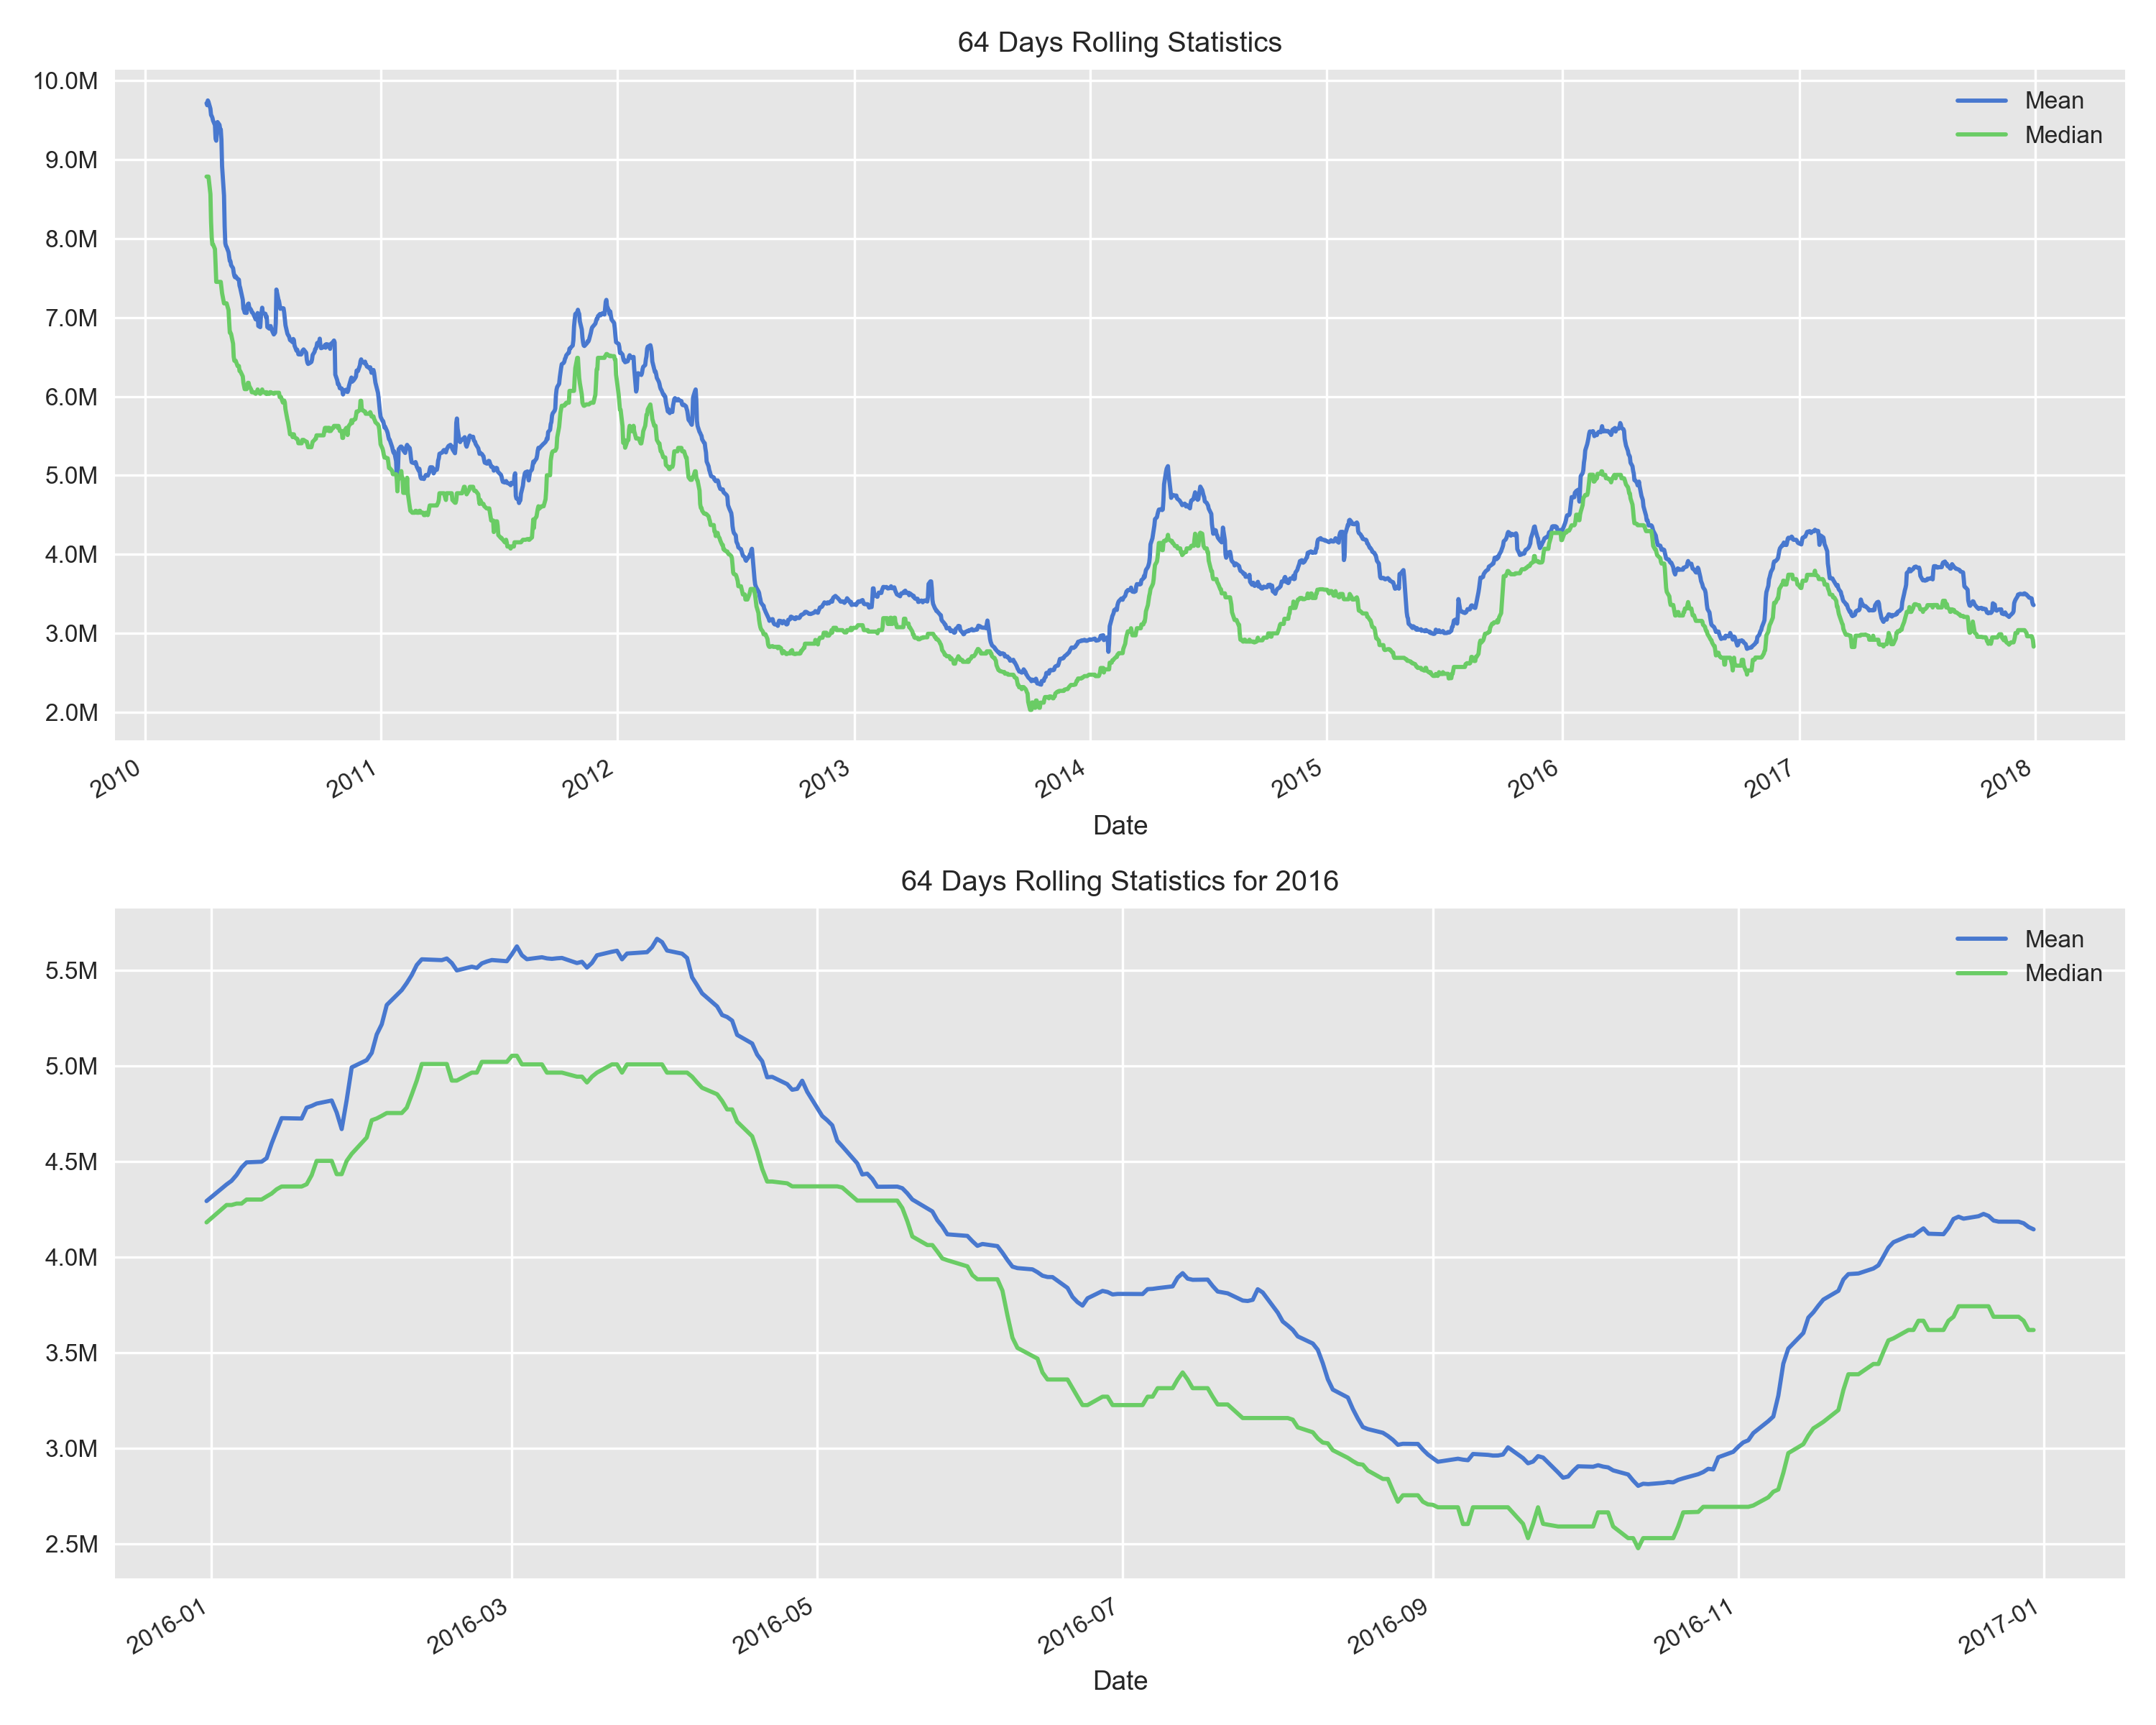
\includegraphics[width=0.75\textwidth]{chapters/chapter_trade_data_models/figures/adv.png} 
		\caption{ADV. Notice how the measure differ. Median is more stable and smooth but Average is more reactive. Which on to use depend on the application\label{fig:adv}}
	\end{figure}

Note that in this section we are only talking about volume as a normalization variable and not a prediction of the day's volume. The two use cases are different although they are often confused. We'll deal with volume prediction in section ?

One of the common uses of relative order size is, as we will see in chapter 10, in the calibration of a market impact model. One would intuitively think that since in the calibration is done after the fact one should normalize using the realized daily volume instead of the ADV. Research has shown that this approach leads to a poorer prediction (any reference?). While the reason for this is not clear it's possible that the large-noise-to-signal ratio is better served by a more stable normalizer vs. a more noisy while more precise one. For consistency reasons using ADV as normalizer in the calibration would imply that we should use of the same normalizer for estimation rather than using our best prediction of daily volume. Practitioners are still debating around this important issue and no research has been done to settle this debate. We'll leave this question to the reader to think about and explore.


\subsubsection{Time-scale Normalization:Characteristic Time }
Trading dynamics have an intrinsic timescale that varies significantly across the stock universe and it is often important to take this into consideration. For instance in a trading algorithm, when evaluating a decision on posting vs. taking (more on that later) , one should estimate what is the likelihood that by posting at the best price the order would get executed before we fall behind our trading commitments. You would not post passively if in average the queue in front for the order takes 3 minutes to clear and you only have 10s before needing to trade. 

A measure commonly used in practice is to look at the median time it takes for the quote to move. This metric is often called Characteristic Time or Turnover Time. 

TODO: formulate this in mathematical terms and implement examples for different liquidity

While more sophisticated approaches are used, which fit more in the HFT alpha signal research we will touch in the next section,having a stable measure that is used in a consistent fashion across the various concerns is highly recommended and leads to a much more stable behavior and improved decision making.

\subsubsection{Intraday Return Normalization: Mid Quote Volatility}
While Characteristic Time answers the question of 'How Long' another common concern is 'How much' meaning how much can the stock in move, in average, over a certain amount of time. As an example if one decides to layer the order book as a way to control adverse selection one should space the order in such a way as to have a consistent behavior across different stocks. Placing the orders the same distance for all stock would cause volatile stock to always execute at multiple level and other more stable stocks the layering would be useless as the deeper orders would rarely execute.  \par 
A common used normalizing variable for and other issues i the Mid Quote Volatility in ticks, estimated as the average number of ticks the mid quote moves in a certain time period or a certain number of characteristic times.

TODO: formulate this in mathematical terms and implement examples for different liquidity


\subsubsection{Microstructure Normalization}
One common mistake of naive trading strategies is trading in a conspicuous and predictable way. Some HFT strategies are trained to spot the presence of large institutional orders so that they can trade ahead of them to build out their inventory they can then sell(buy) back at higher(lower) prices. Since an execution strategy has to trade it's impossible to always be completely invisible to the watchful eye of predatory strategies however with some modest care one can minimize such impact. A common approach use to be less conspicuous is to normalize your actions in so as to avoid changing the average behavior of the stock as measured by various microstructure metrics that are usually closely monitored.  
\begin{itemize}
\item Average Spread: One of the most common microstructure normalizer. TODO Examples. 
\item Average Number Of Trades per second/period: Used as a normalizing variable to control how often one crosses the spread. An noticeable increase in number of trades per second in a certain direction would be read by a predatory strategies as a sign of urgency.
\item Average Trade Size: An unusually large print on exchange or a larger than average block in a dark venue would be spotted  giving our strategy away. One can use the average trade size as a normalizer to decide what size to send to take liquidity.  Note that this measure should in principle be different for different venue types (lit venues, gray venues, dark venues,etc.)
\item Average Quote Size: When the decision to trade passively is made one needs to size the order appropriately. Placing an order that would noticeably change the average size displayed in the inside quote would be interpreted as an directional signal in particular if the size creates a strong imbalance vs the other side (see later on imbalance)
\end{itemize}


\subsection{Intraday Normalization: Profiles}
Incorporating intraday seasonality it's a critical component of competent decision making in execution strategies. Intraday seasonality arise from primarily behavioral and practical reasons around trading discontinutities such as the open and the close (and the lunch break period in certain asian markets) and other scheduled events ( e.g. the US open for European markets). Information dissemination tends to cluster around such times and so then does trading activity. This is compounded by various conventions on how to value certain instruments and other benchmarks. 
  
The standard practice to incorporate this type of seasonality is to normalize decisions via intrarday profiles, essentially functions (usually discrete) that provides the expected value either absolute but more often relative term of some daily measure. While most microstructure variables discussed above showcase some of this seasonality the most used profiles are:
\begin{itemize}
\item Volume Distribution: The percentage of the expected daily volume that will trade in a particular bin.
\item Volatility Distribution: The percentage of the expected daily volatility that will trade in a particular bin.
\item Spread Multiplier: The percentage deviation from the average spread in a particular bin
\end{itemize}

Of particular importance is the Volume Distribution (or profile) as this is the single most important variable used to create a VWAP strategy. For such a strategy, well see, that the volume profile is directly used as the execution schedule for the strategy. This will ensure that the strategy trades a proportionally larger slice of the order at times when more  volume is expected to trade and thus reduce the risk of trading at prices away from the period VWAP.

Volume is most invariably shaped like a flattened U. Volatility and spread both are shaped vaguely exponentially. Volume is clustered around the opening auction(s) and the first several minutes after the open. This makes intuitive sense as the market is re-opening after a trading halt and all new information accrued during the break needs to be incorporated. Spread and Volatility are also large over this period signifying the increased uncertainty around the stock valuation. After this period of heightened activity trading settles in and volume flattens out only to pick up again in the period before the closing auction as investment firms that benchmark to the close price overweight their trading activity to ensure they are receiving price as close to possible to the benchmark without excessive impact. 
\footnote{In this section with ignore the fact that certain markets have lunch breaks. This clearly complicates but does not change the overall picture or approach and it's a relatively trivial extension to the treatment of profiles}. With the recent strong push away from active investing into passive instrument, in particular ETF, the shape of the volume profiles has become increasingly back-loaded to such an extent that almost X%  (TODO Confirm) of the total volume of many stocks happen in the last hour of the trading day 

TODO Show example of smoothed profile both in regular and cumulative terms

\par
Volatilty and spread also have a maximum at the open to account for the uncertainty around the market reaction to  overnight news. As soon as price discovery is finish their value quickly settles and gradually decays to it's minimum at the end of the day.

TODO Show example of smoothed profile both in regular and cumulative terms

\paragraph{Building Intraday Profiles}
Building stable profiles presents non trivial challenges at multiple levels both quantitative, logistical and data related. It will often boil down to matter of trade-offs, data availability, and cost to build and maintain. We provide some, hopefully, valuable pointers that should allow the reader to navigate the hurdles and avoid common pitfalls

\subparagraph{Number of Profile Bins}
As previously mentioned the most common approach for profiles is to use a discrete, piece-wise linear profile. The decision of the numbers of profile bins is a trade-off between required precision and granularity during the most active periods of the day and the lack of stability due to lack of data/change in each bin. One minute bin is the most common choice in the industry.

\subparagraph{Per Stock Profiles vs. Clustered Profiles}
One of the first decisions to be made is whether to create individual profiles for each stock in the universe or use some sort of clustering/grouping. With a universe of several thousand different trading instrument it might be impractical to build and maintain stable individual profiles. Additionally the stability of the profiles is important in order for their use to be effective. Overly illiquid and slowly moving stock will usually make for poor single stock profiles.

A practical and common approach is too use a statistical clustering approach using the L2 norm as distance measure and using a grid search to identify the number of clusters that provides good separation using for example the elbow method (TBD add reference). Given enough clusters 800/900 is not uncommon the outcome of this approach is to have several hundred single element(stock)  clusters for the most liquid and active instruments and a smaller group of clusters that are somewhat related to lower liquidity groups.


\subparagraph{Fitting Approaches}
There are many modeling approaches that are used in practice but there is limited systematic research in this space. 
TODO Add pointers to existing research

First important item is the fitting universe. The common practice is to limit the universe to stocks that would have at least 50-100 trades per bin in every bin. This avoids averaging issues with empty bins.

On the fitting approach, while this would clearly fit within the supervised learning family of methods, this is not necessarily trivial as each bin will have to be treated as an individual variable to allow for the inter-bin variability. There is also auto-correlation among contiguous bins  some additional structure would be warranted. Gaussian Processes look like a promising approach but no research in that direction has appeared as of yet. More often than not no actual fitting takes place but some form of per-bin averaging over a certain length of history after which some form of smoothing is applied.  

TODO What is a good mathematical formulation for the Volume profile Discretized function?

TODO Show an example of Volume profile

Care must be take to remove from the data-set days with predictable differences in profile shape. These "special days" should be modeled separately and we'll provide some pointers in a later paragraph. If one uses some form of regression model the special day could be incorporated as a dummy variable. Other stock specific days like earnings days should also be removed. While in principle  simple process this is in practice not trivial as it's quite hard to have a well organized and maintained special day calendar. This item alone can be the source of a lot of manual labor and cause of frustration and errors. As you'll often see it's not the quantitative aspects that end up being the hardest problems to solve.

\subparagraph{Length of History}
Another common open question is the length of history that should be used. The more data is used the more stable to profiles are however unless great care is given to various seasonal effects and continues changes in market microstructure there is the risk for the profile no to incorporate more recent shifts. This is a particular concern in recent times as the explosion of ETF trading has been consistently shifting more and more volume towards the close. The length of history can be used as a hyper-parameter to be trained on a per cluster basis.

\subparagraph{Volume Profile Smoothing}
intraday volume profiles tend to be extremely noisy and require smoothing to be effective. Some internal research of one of the authors estimated that without smoothing the volume profile performed worse than a completely flat profiles. Care must be taken to avoid smoothing over real discontinuities (e.g. there is a predictable spike in volume in European profiles coincident with the US opening). These spikes usually are preceded by a period of reduced trading activity due to traders waiting for the event. Smoothing these spikes will have the effect of spreading this over previous bins reducing the precision of the profile. One common approach is to remove statistically significant spikes and replace them with a local average for the purpose of smoothing and the re-applying the spike afterward. It has been shown that this approach improves the overall predictability of the profile. 

As far as smoothing algorithms there are a lot of choices available. Kernel smoothing methods have been proven effective. However  care must be given at the boundaries (beginning and end) of the profile. There is a large body of work on how to solve boundary problems in smoothing.

TODO Show an example of smoothed Volume profile vs non smoothed with the jumps removed

\subparagraph{Special Days}
Special days, as previously discussed, present further challenges due to the limited number of data points available (e.g triple witching occurs only 4 time a year). So using larger clusters (one cluster as a limit) is often the only option. One option would be to use these separately calibrated profiles across all special-day clusters. However this would lose the granularity of the regular day clustering. In order to maintain some of the  regular cluster level characteristics a common approach is to use a "difference" profile created by a normalized per-bin ratio between and average regular day profile and the special day profile. This gives a profile that capture the special day systematic shift that can then be multiplied back to the cluster profile essential mixing the two components. While in most cases this has proven effective we would recommend out of sample testing at the cluster level to see i in which profile this is accretive.


TODO Show an example of the Fed-Announcement vol profile

As part of the special day tre

\subparagraph{Dynamic Profiles}
Volume distributions are relatively stable for reasons we have discussed above but they are subject to large distortion due to some 'surprise' event such as unexpected news. In such cases the volume can spike dramatically and the overall realized distribution will end up being highly skewed.  To address this issues sophisticated operator create  dynamic profiles models that take into account the clustering of volume during surprise events skewing the rest of the day's profile more towards the event. There in no academic literature available that studies this problem and most model are proprietary and often heuristic. They also require a sophisticated real-time analytics infrastructure measure and apply these adjustment while the algorithm trades.

As a side note volume spikes and the related distortion of the volume profile is likely still the most common reason why the execution coverage desks get angry calls from clients complaining of their poor. This is because the volume spikes usually happen in conjunction with a a price dislocation and a strategy trading against a static profile would under trade around the event thus leading to a significant deviation from the VWAP benchmark. Of course the coverage desks only hears from the clients on the wrong side of the deviation but never from clients on the positive side! Such is life on the low-touch trading desk.

\section{Remainder of the Day Volume}
A related measure that is of real importance in execution is the Remainder of the day's volume, how much volume are we still expected to see before the market closes. This is of course important for sizing the orders to be sent by investor to avoid excessive impact. It's also important for algorithms that will trade into the closing auction how many shares should be reserved for the auction. We'll discuss more of this in the next section.

So what we are looking for is  $rdv$ then expected cumulative volume from the time $t$ to the end time $T$ :
\begin{equation}\label{eq:rdv_1}
		rdv_t = \mathbb{E} \sum_t^T V_t
	\end{equation}

The most naive approach  is to take the T-1 estimate of today's volume $\tilde{V}_{T-1}$  as discussed in ? and simply remove the cumulative volume up to time $t$

\begin{equation}\label{eq:rdv_2}
		rdv_t ~   \tilde{V}_{T-1} - \sum_0^t V_t
\end{equation}

This approach however almost completely ignores the same day events and, considering how noisy our T-1 estimates tend to be, it leads to relatively poor prediction.

A second approach is at the opposite end of the spectrum and only uses the historical volume profile and the current volume to extrapolate the full day volume and subtract that to the current volume. let $\tilde{X}_t$ the portion of the daily volume expected in bin $t$. Then:

\begin{equation}\label{eq:rdv_3}
		rdv_t ~   \frac{\sum V_0^t}{\sum \tilde{X}_0^t} - \sum_0^t V_t = \sum V_0^t ( ( \sum \tilde{X}_0^t)^{-1} -1)
\end{equation}

This approach is quite commonly used and works reasonably well after 12PM when the activity level is somewhat established. However in the first 2 hours of the day the estimates are quite poor.

The natural  model is to combine the 2 methods essentially using the \ref{eq:rdv_2} as a shrinkage factor with per bin shrinkage factor $\lambda_t$. Thus our model for $rdv$ becomes:

\begin{equation}\label{eq:rdv_4}
	rdv_t ~  \lambda_t( \sum V_0^t ( ( \sum \tilde{X}_0^t)^{-1} -1)) + (1-\lambda)t)(\tilde{V}_{T-1} - \sum_0^t V_t)
\end{equation}

The shrinkage factor $\lambda_t$ is then be calibrated at the bin level to give the best mix of static and dynamic weight. We won't go into the full calibration of this model but only point out some interesting results. As we would expect $lambda_t$ is small at the beginning of the day raising quickly to 70-80\% by noon continuing to increase toward 1 that is reached by construction at the close. What is maybe a bit surprising is that the slope after the initial jump around mid-day is relatively mild meaning that the statis estimate of the daily volume continues to provide stability and a more accurate prediction up until the close. This implies that there is some for of "reversion to the mean" in later parts of the day after some intraday volume surprise.


\section{Auctions Volume}
It is somewhat surprising that so little academic research has been dedicated to such an important aspect of the trading day. I will be even be more surprising the admission that even for practitioners in execution handling the opening and closing auctions is probably a bit more than an afterthought. 

TODO  Max should cover the opening and closing auction mechanics and I'll just reference that
Main concern of this section is the estimation of the auctions volume. This is usually handled as part of the volume profiles estimation in which the opening and closing auctions are respectively the first and last bin of the profile. As per our discussion of volume profiles this ends up being nothing more than an average of the proportion of daily volume. 
thus if $\tilde{X}_0$ and $\tilde{X}_T$ the T--1 opening and closing volume are measured by 

Section ? already covered the mechanics of the opening and closing auctions so we will not cover them again here.



As mentioned multiple times the current growing trend towards passive investments and ETF has driven the liquidity more and more towards the close. This means that the closing auction is becoming more and more the center of liquidity management.  It's quite likely that no other area of research is more relevant and impact-full that focusing on better understanding the closing period in price and volume dynamics in particular in relation to the create-redeem activities and the  cross-asset classes dynamics.


\section{Microstructure Signals and other Advanced Analytics}
This is not a book revealing secret alpha signals. But no coverage of the subject would be close to complete if at least we don't cover more advanced topics in microstructure signals. Again the subject is quite extensive and academic literature is almost non existent since any successful research in the space can be utilize in practice and thus unlikely published. Here we just gave a brief overview of common signals utilized in practice as a starting point for the interested researcher/practitioner.

\subsection{Quote Imbalance}
Arguably the most used microstructure signal used by practitioner and still one of the most predictive ones is the quote imbalance.  The simplest measure of quote imbalance can be defined as: 
	\begin{equation}\label{eq:q_imb}
		qimb = \frac{bs - os}{os + bs}
	\end{equation}

The intuition behind why quote imbalance is predictable of the next quote movement is simple: if more and more buyers enter the market before crossing the spread they will likely try their luck by posting a the best bid. The more people pile up the more unlikely that they will find a seller and eventually one of the buyers will run out of patience and cross the spread. If the opposite size is small (i.e. the quote imbalance is heavily slanted toward the buy side it's likely the trade will clear the price level leading to a price move.

\subsection{Book Imbalance}
More sophisticated measures of the imbalance considers not only the inside quote but the whole book. A simple version would be some form of weighted average across multiple levels and would look something like: 
	\begin{equation}\label{eq:microprc}
		obimb = \frac{1}{N}\sum_{i=0}^Nw_i (bs_i-os_i)
	\end{equation}

where $w_i$ would be a function of the distance of the $i$ price point (possibly normalized by the quote volatility) and $N$ is some appropriate normalization.

\subsection{Microprice}
a common simple approach to incorporate quote imbalance in a 'fair' price is to consider the quote adjusted mid point often called Microprice. This is defined as:
	\begin{equation}
		\frac{os bp + bs op}{(os+bs)}
	\end{equation}

The microprice as the following intuitive characteristics: 
\begin{itemize}
\item For 0 imbalance the microprice is equal to the mid price
\item For positive imbalance the microprice tends to ask price implying the fair price is higher thatn the midprice
\item For negative imbalance the microprice tends to bid price implying the fair price is lower than the midprice
\end{itemize}

	\begin{figure}[!ht]
		\centering
			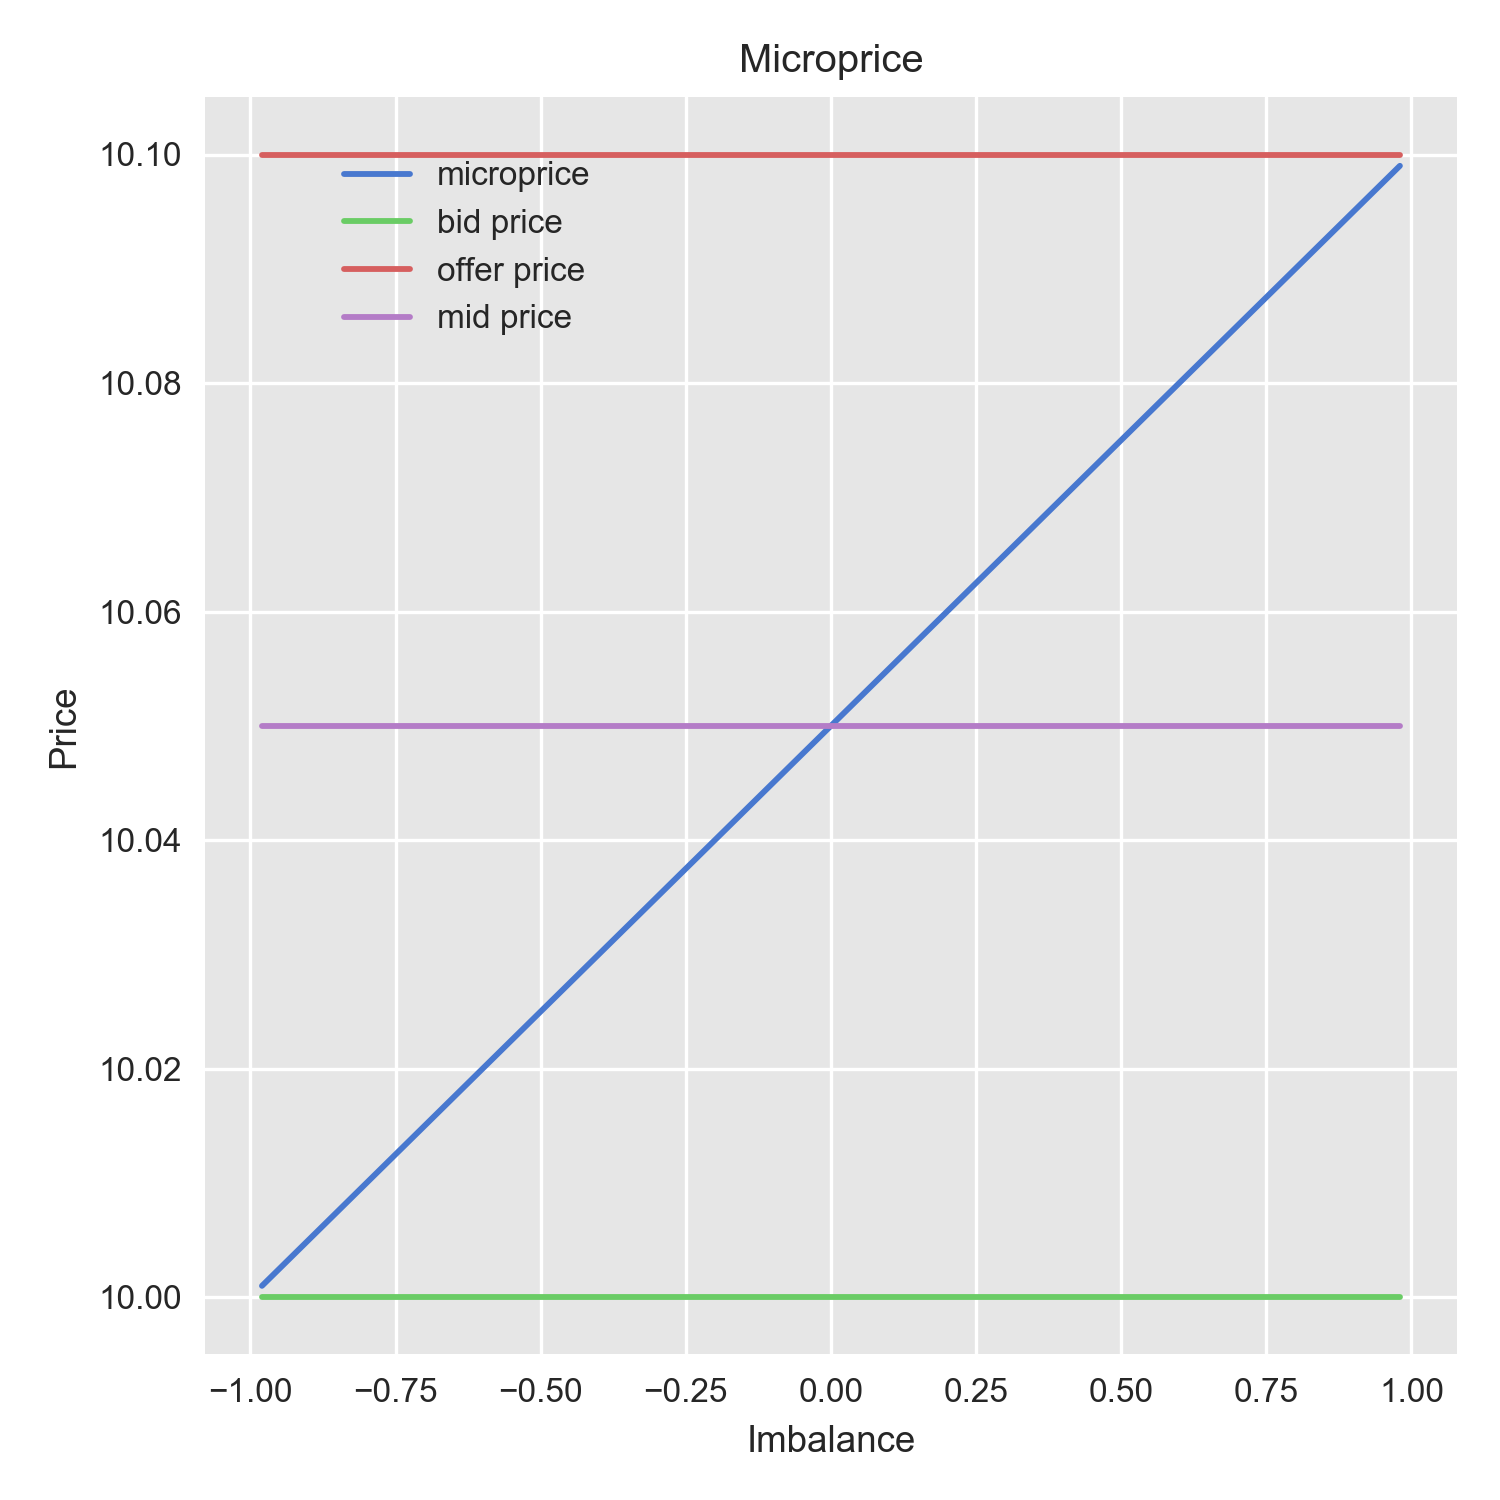
\includegraphics[width=0.75\textwidth]{chapters/chapter_trade_data_models/figures/microprice.png} 
		\caption{Microprice. for different levels of imbalance. \label{fig:microprice}}
	\end{figure}

One can easily envision other microprices that incorporate Order book imbalance as well as the impact of the last traded price.

\subsection{Trade Imbalances}
For every trading transaction there is always on side that is the initiator of the trade, in general the counterpart that ran out of patient and decided to pay the spread. This implies either some informed trader or a trader that has some urgency because it has a lot more to do. In either case an imbalance between the amount of buyer initiated volume vs. seller initiated volume would likely be instructive. One way to define trade imbalance is: 

	\begin{equation}
		\frac{V_b}{V_b+V_o}	
	\end{equation} 

A 1(0) trade imbalance would mean that all the volume was buy(sell) initiated. 

While this is very simple metric the challenge is: How do I categorize a trade as buyer/seller initiated? For most practitioner who do not have access to Level III data and only has quotes and trades this is a lot trickier than one would think and there is a discrete amount of research around the efficacy of various algorithms. If one has Level III this information is trivial to identify for lit venues. However this is not the case for dark venues were the trade classification of large blocks could be quite valuable.

Me most popular approach for trade classification was proposed by Lee and Ready 2010)~\cite{leeready} with subsequent revisit by ~Chakrabarty, B. and Moulton, P. C. and Shkilko, A. (2012)~\cite{chakrabarty2012short}

The simplest version of this algorithms goes approximately like this:
\begin{itemize}
\item If the execution price is $gt$ the prevailing mid price the trade is buyer initiated
\item If the execution price is $lt$ the prevailing mid price the trade is seller initiated
\item If the execution price is equal to the prevailing mid price the trade market as the previous trade
\end{itemize}

The algorithms has proven only moderately predictive to  ~75\% accuracy. This is due to various causes. One such cause due to the asynchronous nature of the trade and quote streams and where a quote change could be time stamped slightly before the trade that affected it leading to mis-classification.

\section{Advanced Models}
TODO We might want to re-organize this so we have the more practitioner treatment in part 1 of the chapter and then more advanced features like the below and we can add more as needed.

\subsection{Models for LOB dynamics}

Before we formally present the models, we want to provide a review of how the analysis of LOB data has been approached. Biais, Hillion and Spatt (1995)~\cite{spalt} study the trading activity in Paris Bourse (a fully automated limit order market), the dynamics of order flow and how the order flow varies with the state of the order book and marketplace events relevant to the asset. It is found that the conditional probability of a limit order placement is larger when the bid-ask spread is larger and when the order book is not deep. If a market order has been placed the chance that the next order posted provides liquidity is generally higher. The placement of orders also follows a pattern with new orders coming in the morning when the price discovery occurs and cancellations and large orders occur in the evenings. The durations between trades do indicate that the intensity of trade varies during the course of a day. The main tool used in these calculations is contingency table which provides both marginal and conditional probabilities. \\

\noindent \textbf{Slope of LOB:} To begin with we can consider the slope of the order book both on the demand side and on the supply side using the quotes on both sides various depths (see Figure~\ref{fig:limitstocks}). This provides information on order book imbalance that can be helpful for the trader to decide on the optimal time to enter or to exist the market (see Figure~\ref{fig:limitstocks}). It is observed from Figure~\ref{fig:limitstocks} that the bid-ask spread is at least twice the difference between quotes at successive depths. Thus the slope of the book is steeper closer to the best quotes. \\
	\begin{figure}[!ht]
	   \centering
	   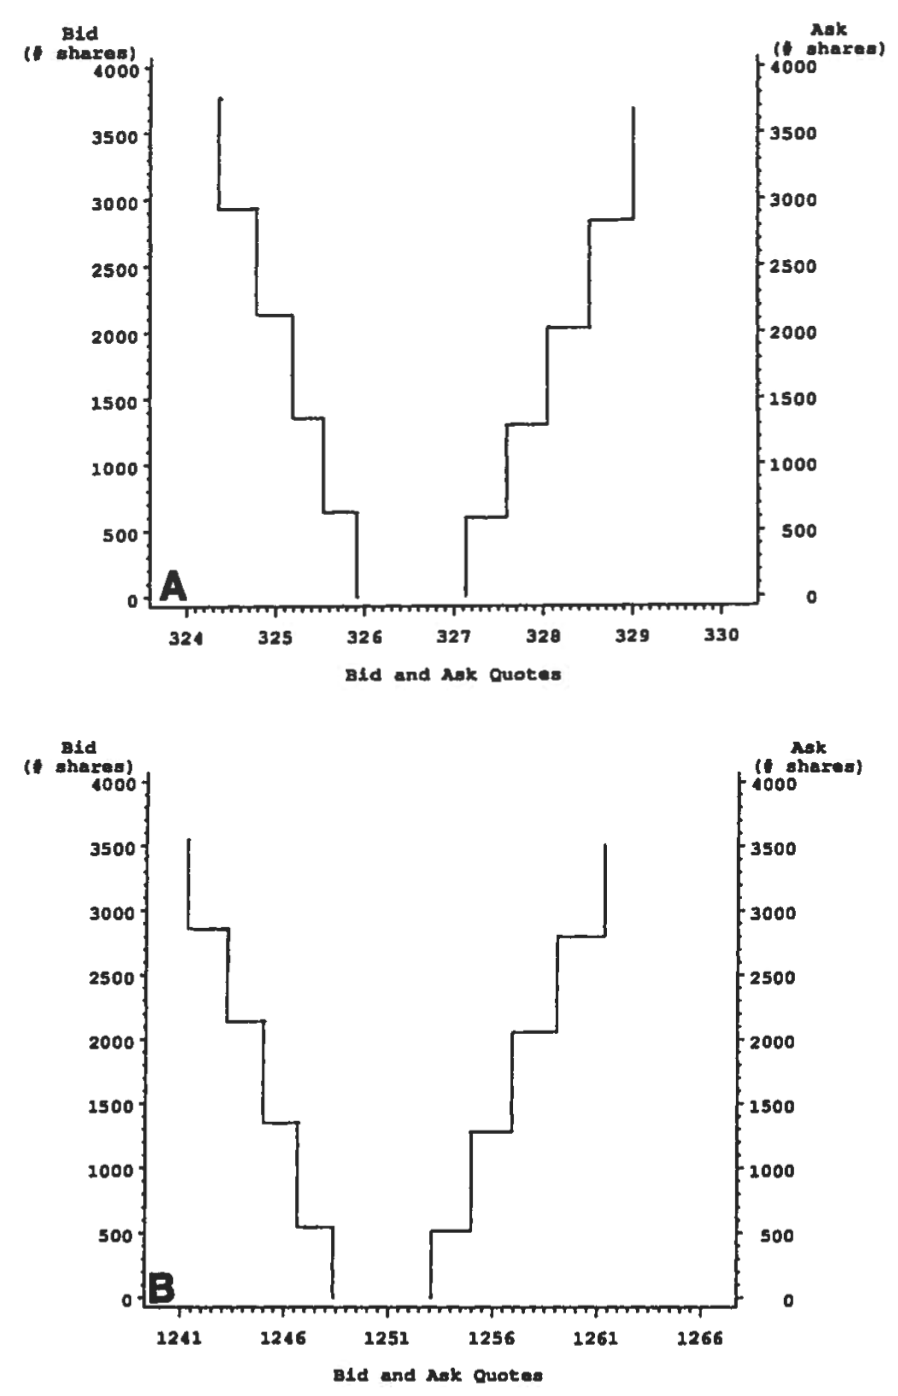
\includegraphics[width=0.75\textwidth]{chapters/chapter_trade_data_models/figures/limitstocks.png} 
	\caption{The Limit Order Book for Stocks. (A) Plots the cross-sectional average (across with tick$=$FF 0.1) of the time-series averages of the five best ask and bid quotes and their associated depth. (B) plots the cross-sectional average (across stocks with tick$=$FF 1) of the time-series averages of the five best ask and bid quotes and their associated depth.\label{fig:limitstocks}}
	\end{figure}

\noindent\textbf{Order Flow:} The orders can be characterized as buyer or seller initiated and how aggressive they are. The aggressiveness is quantified by the size of the order. Most of the orders are small indicating that they could be part of a large parent orders. Both placement and cancellation of orders seem to decrease away from the best quotes. As the intra-day trading pattern follows typical diurnal pattern, both the depth and order flow must be adjusted for the time of the day. Some observations (stylized facts) worth noting are:
\begin{enumerate}[--]
\item Large (small) trades on one side of the market tend to be followed by large (small) trades on the same side. The same thing could be said about the new limit orders and cancellations as well. It is speculated that this may be due to traders reacting similarly to the same events or due to parent order splitting and automatic placement of child orders. \\

\item Cancellations on the buy side of the book are more frequent after market buy orders and the same for sell orders. This may be due to the fact that the large sell orders tend to convey negative information about the stock while the large buy orders convey positive information. Cancelations may also occur because of placement of some market orders are intended to probe the presence of any hidden orders. \\

\item Conditioning on the state of the book by size of bid-ask spread and the depth, it is observed that trades are more frequent when the spread is tight but the new orders inside the quotes are more frequent when the spread is large. The changes in spread are mainly due to liquidity shocks. \\

\item Frequency of trades tends to be clustered because competing traders who monitor the market closely are likely to place the orders when they read the market in their favor. It is observed that the trading activity is more intense with the information flow. Also observed are the following stylized facts: when the spread is large after liquidity shocks, traders place their orders quickly to take advantage of time priority. Thus the spread reveals back to original level. The expected time interval is generally lower after large trades than after other trades whether the spread is large or not.
\end{enumerate}


Thus the study by Biasis et al. (1995)~\cite{spalt} provides a set of concrete measures that could be used to study the dynamics of the limit order book. Now we will delve into model formulations. 


One of the earlier models to appear in the econometric literature is by Lo, MacKinlay and Zhang (2002)~\cite{maczhang}; they used the data from Investment Technology Group (ITG) that contained time stamped information on each limit order from submission to cancellation or execution. With three possible paths for each submitted order, the associated (a) time-to-cancellation/modification, (b) time-to-first fill and (c) time-to-completion are tracked and models are developed for each path on both sides of the order. Because ITG largely deals with the institutional investors, the results apply only to a limited segment of the traders. The modeling approach is to get the execution times as the first-passage time to the limit price assuming that price follows a geometric Brownian model with a drift (Model 1.1):  
	\begin{equation}\label{eqn:dp(t)}
	dP(t)= \alpha \cdot P(t) \; dt + \sigma \cdot P(t) \; dW(t)
	\end{equation}
where $W(t)$ is a standard Brownian motion. A buy limit order with a price `$P_l$' is executed in the time interval $[t_0,t_0+t]$ only if $P_{\text{min}} \leq P_l$ and the probability is
	\begin{equation}\label{eqn:expprob}
	P_r(P_{\text{min}} \leq P_l \;|\; P(t_0)=P_0)= 1- \left(1 - \left(\dfrac{P_l}{P_0}\right)^{2\mu/\sigma^2}\right) \Phi\left[\dfrac{\ln(P_0/P_l) + \mu t}{\sigma \sqrt{t}}\right]
	\end{equation}
where $\mu=\alpha - \frac{1}{2} \sigma^2$ and $\Phi(\cdot)$ is the cumulative distribution function of the standard normal. 

Note (\ref{eqn:expprob}) can be alternatively stated as, if `$T$' denotes the limit order execution time, $F(t)=P(T \leq t \;|\; P_0)$ for buy orders and similarly for sell orders, $F(t)=p_r(P_{\text{max}} \geq P_l)$. To see if the model is appropriate for the data at hand compare the theoretical c.d.f. of $F(t)$ to empirical c.d.f. using the well-known result that these are uniformly distributed. Fix `$\tau$' as the fixed sampling interval and with $r_t=\ln(P_t)-\ln(P_{t-1})$, the estimates of $\mu$ and $\sigma^2$ are:
	\begin{equation}\label{eqn:sampleestm}
	\hat{\mu}= \dfrac{1}{N\tau} \sum_{j=1}^N r_j, \quad \hat{\sigma}^2= \dfrac{1}{N} \sum_{j=1}^N \dfrac{(r_j - \hat{\mu} \tau)^2}{\tau}
	\end{equation}
where `$N$' is the number of observations in the sample. 


The above First Passage Time (FPT) model was used for filled orders without taking into account that other orders that were cancelled or modified in that duration. The model's other limitations include not accounting for time priority, not including other relevant variables such as price volatility, spreads, etc.. The model's performance using the empirical cumulative distribution function is shown to be lacking. The model (\ref{eqn:expprob}) is expanded as
	\begin{equation}\label{eqn:cumexpmodel}
	F(t)=p_r(T_k \leq t \;|\; X_k,P_{lk}, S_k, I_k)
	\end{equation}
where $T_k$ is the execution of time of $k$ orders, $P_{lk}$ is the limit order price, $S_k$ is the size and $I_k$ is the side indicator. An alternative function, the hazard rate (briefly discussed in Chapter 2)
	\begin{equation}\label{eqn:hazard}
	h(t)=\dfrac{f(t)}{1-f(t)}= \dfrac{f(t)}{S(t)}
	\end{equation}
is found to be useful to operationalize and explain the modeling of survival rate of time-based events; Note $S(t)$ is called the survivor function. The censoring information ($\delta_i=1$ if observation `$i$' is censored) can be incorporated with $t_i$, $i$th realization of the random variable, $T$. It is assumed that the censoring mechanism is independent of the likelihood the limit order is executed. Using the generalized Gamma (defined in Chapter 2) as $f(t)$, the models are estimated.


The following variables are used as explaining variables:
\begin{enumerate}[--]
\item Distance between mid-quote and limit price.
\item Prior trade indicator for buyer or seller initiated.
\item Measures of liquidity.
\item Measures of market depth.
\item Measures that reflect change in trading activities. 
\end{enumerate}
It is shown that this model does fare better than FPT model to capture the execution times. But an important limitation is ``\dots censoring as a result of prices moving away from the limit price would be a violation of the underlying assumption since prices at the time of censoring are not included in $X_i$.'' We show in our analysis of Level III data, a key determinant for cancellation of an order is that price moving away from the limit price that the trader has desired. 


There are a number of studies that have looked into order book dynamics using models that arise from Point Processes. Bouchard, Mezard and Polters (2002)~\cite{bouchardmezard} investigate the interaction between order flow and liquidity; it is observed that the distribution of incoming limit order prices follow a power law around the current price and the overall shape of the book in terms of volume on both sides is rather systematic. Smith, Farmer, Gillemot and Krishnamunthy (2003)~\cite{smithfarm} and Farmer et al. (2004)~\cite{} study how the order flow influences price formation; the price impact of market orders is a function of touch price depth and spread size. Hewlett (2006)~\cite{} focuses on using LOB dynamics to find optimal liquidation strategies in foreign currency markets. 


To have a more complete and realistic picture of how the LOB evolves, we must consider `hidden liquidity'. Almost all exchanges allow traders to hide all or portions of their orders. The so called, ``iceberg order'' is split into several smaller parts and is queued along with the other orders, but only the displayed quantity is visible and is part of the market depth. When the order reaches the front of the queue only the displayed is executed. Several reports could be as high as 26\%. In the models discussed below, we will not address the hidden liquidity issue, which will be taken up in a later section.


Modeling of LOB dynamics has drawn on ideas from economics, physics, statistics and psychology. The approach taken in economics literature is to focus on the behavior of the traders and the dynamics is modeled as sequential games (Foucault (1999)~\cite{}, Parloys (1998)~\cite{} and Rosu (2009)~\cite{}). Others, such as researchers from physics, have treated order flows as random and statistical mechanics techniques are used to study the dynamics. Other studies, such as Parlour and Seppi (2008)~\cite{parseppi} and Bouchaud et al. (2009) are useful references for studies that come from economics point of view. We will review three models that are of recent origin. \\


\noindent\textbf{Cont, Stoikov and Talreja (2010)~\cite{contstoi}}: In this model of the limit order book, the number of limit orders at each price level in the book is taken to be a continuous-time Markov chain. The evolution of the order book through market orders, limit orders and cancellations is represented as a counting process. The model replicates the evolution of the events using independent Poisson processes. The study views LOB as a system of queues subject to order book events whose occurrences are modeled as a multidimensional point process. Before we state the specific questions and the models implications, we define certain useful quantities. 


It is taken that the price grid as $P(n)=\{1,2,\ldots,n\}$ multiples of a price tick. The number of outstanding orders in the book $|X_t^i|$ at price $i$, collectively, $X_t \equiv (X_t^1,\ldots,X_t^n)$ is taken to be continuous-time Markov chain; if $X_t^i<0$, then there are $-X_t^i$ bid orders at price `$i$' and if $X_t^i>0$, then there are $X_t^i$ ask orders at price $i$. Now we have,
	\begin{equation}\label{eqn:bestmidspread}
	\begin{split}
	\text{Best Ask Price: }& p_A(t)=\inf\{i \colon X_t^i>0\} \\
	\text{Best Bid Price: }& p_B(t)=\sup\{i \colon X_t^i<0\} \\
	\text{Mid Price: }& p_M(t)=(p_A(t)+p_B(t))/2 \\
	\text{Spread: }& p_S(t)=p_A(t)-p_B(t)
	\end{split}
	\end{equation}
The depth of the order book is stated relative to best bid and best ask on either side of the book. This way the model can be applied to order book for any equity subject to ever changing, best bid and best ask. Define
	\begin{flalign}\label{eqn:qaqb}
	&& Q_i^B(t)&= \begin{cases} X_{p_A(t)-i}(t), & 0<i<p_A(t) \\ 0, & p_A(t) \leq i <n \end{cases} && \notag \\
	\text{and} && \phantom{x} & \phantom{x} && \\
	&& Q_i^A(t)&= \begin{cases} X_{p_B(t)-i}(t), & 0<i<n-p_B(t) \\ 0, & n-p_B(t) \leq i <n \end{cases} && \notag
	\end{flalign}
Thus, $Q_i^B(t)$ and $Q_i^A(t)$ denote the number of buy orders at a distance `$i$' from ask and the number of sell orders at a distance `$i$' from bid, respectively. This representation highlights the shape (or depth) of the book relative to the best quotes on either side.


The following assumptions are made on the order arrivals: market buy or sell orders arrive at independent exponential times with rate, $\mu$. Limit buy or sell orders arrive at a distance of `$i$' ticks from the opposite best quote at independent exponential times with rate $\lambda(i)$. The cancellations of limit orders occur at a rate proportional to the number of outstanding orders, $\theta(i)X$. All these events are assumed to be mutually independent.


How the limit order is updated with the inflow of above events can be described as follows: for a state $x \in \mathbb{Z}^n$ and $1 \leq i \leq n$, let $x^{i \pm 1}=x \pm (0,\ldots,1,\ldots,0)$, where `1' denotes the change in the $i$th component. For example, a limit buy order at price level, $i<p_A(t)$ increases the quantity at level `$i$', from $x$ to $x^{i-1}$ with rate $\lambda(p_A(t)-i)$. Similarly, limit sell order arrived which changes the order book from $x$ to $x^{i+1}$ with rate $\lambda(i-p_B(t))$ for $i>p_B(t)$. For market buy order decreases at the ask price $i$ and hence $x \to x^{p_A(t)+1}$ with rate `$\mu$' and the sell order at the bid price, `$i$' will change the book status, $x \to x^{p_A(t)+1}$ with rate $\mu$. Cancellation of a buy order at price level, `$i$', will decrease the quantity at the rate $\theta(p_A(t)-i)|X_p|$ for $i<p_A(t)$ and the sell order will decrease the quantity at the rate of $\theta(i-p_B(t))|X_p|$ for $i>p_B(t)$.


It is assumed that the limit order arrival rate $\lambda(i)$ follows a power law
	\begin{equation}\label{eqn:powerlaw}
	\lambda(i)=\dfrac{\kappa}{i^\alpha}
	\end{equation}
which is confirmed by several empirical studies (Farmer (2002)~\cite{} for example). The empirical estimates of the parameter are based on the following quantities: $s_m$ is the average size of the market orders, $s_l$ is the average size of the limit orders and $s_c$ is the average size of the cancelled orders. Also let $N_l(i)$ be the total number of limit orders that arrived at a distance `$i$' from the opposite best quote and $T_*$ is the total trading time in minutes and $N_m$ is the number of market orders during the sam time. Then 
	\begin{equation}\label{eqn:hatlambdant}
	\hat{\lambda}(i)= \dfrac{N_l(i)}{T_*}, \quad 1 \leq i \leq 5
	\end{equation}
where $\hat{\lambda}(i)$ is extrapolated beyond five positions using the power law in (\ref{eqn:powerlaw}) simply by minimizing $\sum_{i=1}^5 (\hat{\lambda}(i)- \frac{\kappa}{i^\alpha})^2$, over `$\kappa$' and `$\alpha$'. The arrival rate is estimated as:
	\begin{equation}\label{eqn:hatnmt}
	\hat{\mu}=\dfrac{N_m}{T_*} \cdot \dfrac{s_m}{s_l}
	\end{equation}
The cancellation rate as noted earlier is defined as proportional to the number of order at that price level,
	\begin{equation}\label{eqn:hatthetacase}
	\hat{\theta}(i)=
	\begin{cases}
	\dfrac{N_l(i)}{T_*Q_i} \cdot \dfrac{s_c}{s_i}, & i \leq 5 \\
	\hat{\theta}(5), & i>5
	\end{cases}
	\end{equation}
It is understood that the cancellation is not due to executing market orders.


While these descriptives are easy to compute and are intuitive, but the main interest in modeling high frequency dynamics of order book is to predict short-term behavior of various key quantities that were identical earlier that may help in algorithmic trade executions. Some relevant questions are as stated before, given the state of the order book, what is the probability that mid-price will move up, what is the probability of executing both buy and sell order at the best quotes before the price changes etc.. These conditional probabilities are evaluated using Laplace transforms.


We present some key results in Cont et al. (2010)~\cite{contstoi}. The probability of queue going up when there are no orders in the queue, for $1 \leq d \leq 5$, given that the best quotes are not changing is
	\begin{equation}\label{eqn:queuecon}
	p_{\text{up}}^d(m)=
	\begin{cases}
	\dfrac{\hat{\lambda}(d)}{\hat{\theta}(d)m+\hat{\lambda}(d)+\hat{\mu}}, & d=1 \\
	\dfrac{\hat{\lambda}(d)}{\hat{\theta}(d)m+\hat{\lambda}(d)}, & d>1.
	\end{cases}
	\end{equation}
Other questions such as the probability that the mid price goes up when the spread $\geq 1$ etc. are based on the following quantities:
\begin{itemize}
\item Probability of a market buy order
	\begin{equation}\label{eqn:probmarketbuy}
	\dfrac{\mu^a}{\mu^b+\mu^a+\sum_j (\lambda_B(j)+\lambda_A(j)+\theta(j) Q_j^A(t)+\theta(j)Q_j^B(t))}
	\end{equation}
\item Probability of a limit buy order $d$ ticks away from the best ask
	\begin{equation}\label{eqn:problimitbuytick}
	\dfrac{\lambda_B(d)}{\mu^b+\mu^a+\sum_j(\lambda_B(j)+\lambda_A(j)+\theta(j)Q_j^A(t)+\theta(j)Q_j^B(t))}
	\end{equation}
\item Probability of a cancel buy order $d$ ticks away from the best ask
	\begin{equation}\label{eqn:probcanceltick}
	\dfrac{\theta(d)Q_d^B(t)}{\mu^b+\mu^a+\sum_j(\lambda_B(j)+\lambda_A(j)+\theta(j)Q_j^A(t)+\theta(j)Q_j^B(t))}
	\end{equation}
\end{itemize}
The model was evaluated using data sets from Tokyo Stock Exchange. The model is shown to capture realistic features of the order book profile.
	\begin{figure}[!ht]
   	\centering
   	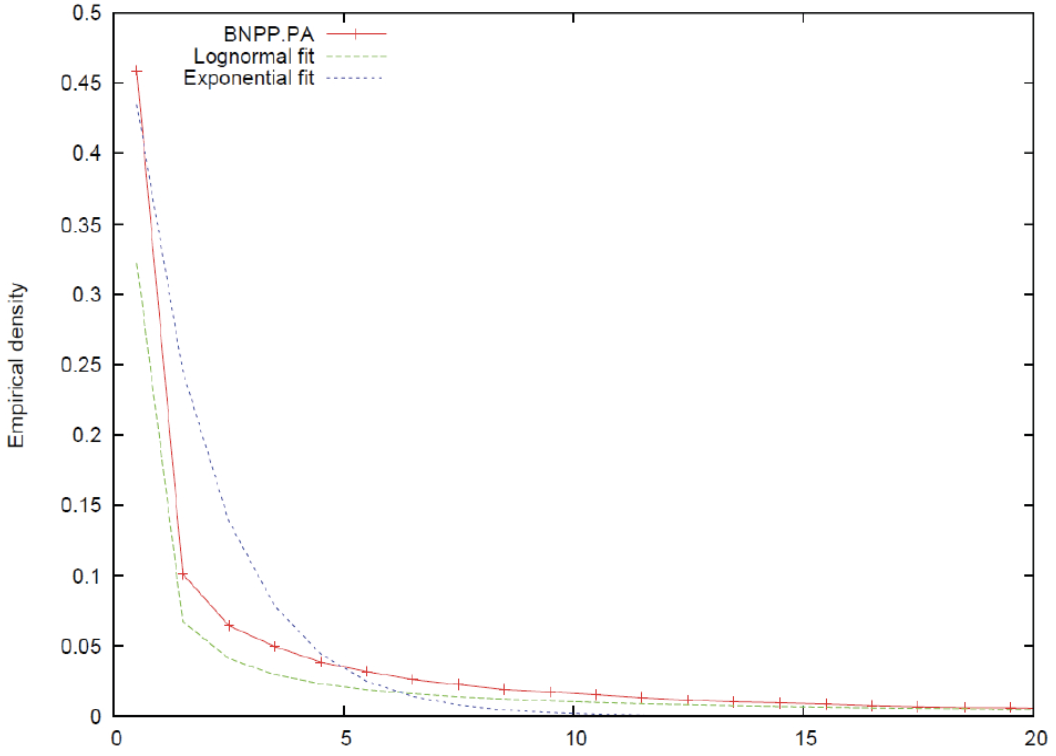
\includegraphics[width=0.9\textwidth]{chapters/chapter_trade_data_models/figures/intertime.png} 
   	\caption{Distribution of inter-arrival times of market orders for stock BNPP.PA (Chakraborti et al. 2011). \label{fig:intertimefig}}
	\end{figure}

The use of Poisson processes to model the flows of limit orders, market orders and cancellations makes the method analytically tractable. The model captures the steady-state shape of the order book (although there may be other distributions that may be fit better besides Poisson, see Figure~\ref{fig:intertimefig}) but it may not be useful for predicting short-term behavior that may be more relevant for the traders. The assumption of Poisson process results in that the intensity of arrivals and cancellations does not depend on the state of the order book which is somewhat unrealistic given the feedback loop relationship between the behavior of the market participants and the history of the order book. Recent works, by Zhao (2010)~\cite{} and Abergel (2010)~\cite{} show that the memory-less property is not empirically valid. Orders tend to be clustered due to dependencies between liquidity taking and liquidity providing and also due to algorithmic execution of parent order that is split into numerous child orders. Also, the assumption that all orders are of the same size is too simplistic. 


Zhao (2010)~\cite{} proposes a model based on marked point process when the mark represents order types, price, size etc.. The joint modeling also assumes that the order flow is self-exciting, i.e. new orders or cancellations occur in an orderly point processes with an intensity function that depends on the history of the limit order book. The model is somewhat difficult to estimate and does not fully capture the empirical results such as volatility clustering etc.. \\

\noindent\textbf{Hawkes Process:} The features of volatility clustering and the significant autocorrelations in durations between order arrivals and significant cross-correlation of arrival rates across various event types are better captured by multi-dimensional Hawkes process. For a given $M$-dimensional point process, let $N_t=(N_t^1,\ldots,N_t^M)$ denote the associated counting process and the Hawkes process is characterized by intensities, $\lambda^m(t), m=1,\ldots,M$ as
	\begin{equation}\label{eqn:lambdamdoub}
	\begin{split}
	\lambda^m(t)&= \lambda_0^m(t) + \sum_{n=1}^M \int_0^t \sum_{j=1}^P \alpha_j^{mn} e^{-\beta_j^{mn}(t-s)} dN_s^n \\
	&=\lambda_0(t) + \sum_{n=1}^M \sum_{t_j<t} \sum_{j=1}^P \alpha_j^{mn} e^{-\beta_j^{mn}(t_j -t_i^n)}
	\end{split}
	\end{equation}
where the number of exponent kernels, $P$, is fixed and $t_i^n$ is the $i$th jumping time of the $m$th variate. The scale and decay parameters, $\alpha^{mn}$ and $\beta^{mn}$ express the influence of the past events $t_i^n$ of type `$n$'. The baseline model in (\ref{eqn:lambdamdoub}) does not incorporate the effect of bid-ask spread on order flow. It is shown in Anderson, Cont and Vinkovskaya (2010)~\cite{} that $\alpha$ and $\beta$ parameters do depend on the bid-ask spread. A simulated Hawkes process is given in Figure~\ref{fig:hawkes}. The main characteristic of the Hawkes process is that intensity goes up at each event and decays exponentially between events. 
	\begin{figure}[!ht]
   	\centering
   	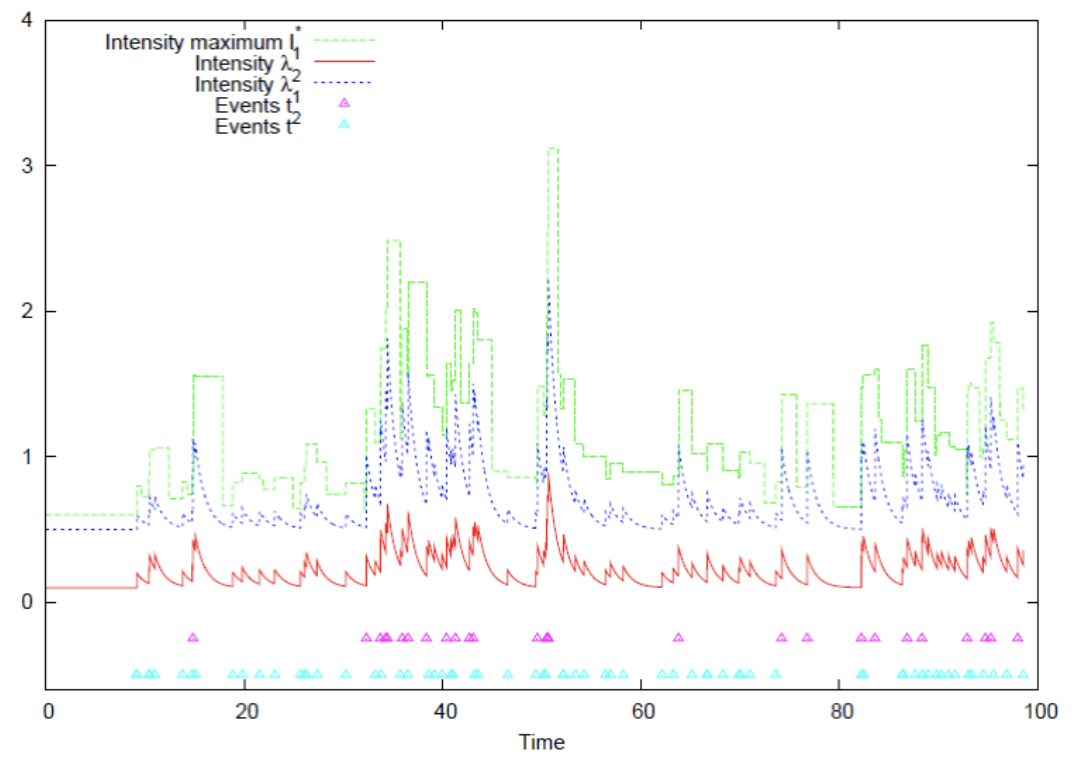
\includegraphics[width=0.9\textwidth]{chapters/chapter_trade_data_models/figures/hawkes.png} 
   	\caption{Simulated two-dimensional Hawkes process (Toke 2011). \label{fig:hawkes}}
	\end{figure}

The evolution of the order book is driven by six different intensity functions, but the model changes with the value of the spread. The base intensity and the decay rates are all assumed to be functions of the spread. The model is quite complex and requires the estimation of a large number of parameters, which in turn requires vast amount of data for calibration. 


The mathematical framework was developed in Hawkes (1971)~\cite{} and was expanded in Hawkes and Oakes (1974)~\cite{}. The application of Hawkes process in finance is of recent origin: see Toke (2011)~\cite{} or Bacry et al. (2011)~\cite{}. We will briefly discuss the likelihood estimates of the model in (\ref{eqn:lambdamdoub}). First, we want to observe for a Poisson process, the intensity function $\lambda(t)=\lambda_0$, a constant. The log-likelihood of the model,
	\begin{equation}\label{eqn:loglikemod}
	\ln \mathcal{L}(\{t_i\}_{i=1,2,\ldots,N}) = \sum_{m=1}^M \ln \mathcal{L}^m(\{t_i\})
	\end{equation}
where
	\[
	\ln \mathcal{L}^m(\{t_i\})= T - \sum_{i=1}^N \sum_{n=1}^M \dfrac{\alpha^{mn}}{\beta^{mn}} (1- e^{-\beta^{mn}(T-t_i)}) + \sum_{t_i^m} \ln[ \lambda_0^m(t_i^m) + \sum_{n=1}^M \alpha^{mn} R^{mn}(l) ]
	\]
and 
	\[
	R^{mn}(l)= \sum_{t_\kappa^n t_l^m} e^{-\beta^{mn}(t_l^m-t_\kappa^n)}
	\]
is the cumulative decay function. Using the Multiplicative Random Time Change Theorem (see Meyer (1971)~\cite{}) that states that with a certain transformation of the variables, the Hawkes process can be changed to a unit rate homogeneous Poisson process. Transforming the time variable `$t$' into `$\mathcal{T}$', where
	\begin{equation}\label{eqn:calt}
	\mathcal{T}= \int_0^t \lambda(s) \; ds
	\end{equation}
Hawkes process becomes a Poisson process with unit rate. Thus
	\begin{equation}\label{eqn:diffcalt}
	\mathcal{T}_i - \mathcal{T}_{i-1}= \Lambda(t_{i-1},t_i) = \int_{t_{i-1}}^{t_i} \lambda(s) \; ds
	\end{equation}
is exponentially distributed. 


More generally in the `$M$' dimensional multivariate case,
	\[
	\begin{split}
	\Lambda^m(t_{i-1}^m,t_i^m)&= \int_{t_{i-1}^m}^{t_i^m} \lambda_0^m(s) \; ds + \int_{t_{i-1}^m}^{t_i^m} \sum_{n=1}^M \sum_{t^n<t_{i-1}^m} \alpha^{mn} e^{-\beta^{mn}(s-t^n)} \; ds \\
	&+ \int_{t_{i-1}^m}^{t_i^m} \sum_{n=1}^M \sum_{t_{i-1}^m<t^n<s} \alpha^{mn} e^{-\beta^{mn}(s-t^n)} \; ds
	\end{split}
	\]
will follow exponential distribution. The $\Lambda^m(t_{i-1}^m,t_i^m)$ are known as compensators and can be verified empirically if it follows exponential distribution. 


\subsubsection{Application of a Hawkes process}


We want to illustrate the model with an application. We will first look at the statistical properties of the data and then look at the results of fitting one and two dimensional Hawkes processes to it. Our findings show that a two dimensional model based on Hawkes processes performs considerably better than a model based on two independent Poisson Processes. This provides strong evidence of the fact that the two key features of Hawkes processes (path dependency of the order flow and the possibility of modeling the interaction between the dimensions) are capable of capturing and replicating some of the key features of the empirical data. Moreover, there is evidence of significant and asymmetric interplay between the buy and the sell sides for the Limit Orders and evidence of limited interplay between the two sides when it comes to Market Orders. Finally, a study of the statistical properties of the orders showed a complex of alternating symmetric and asymmetric behavior of the LOB. 


The data at hand is INET data for XOM (Exxon Mobil) for the 1st of September 2010. The first step was to look at the submission frequency of the Limit Orders during the trading day. Figure~\ref{fig:freqsubmitarrivals} shows such frequency plot and we can see how in the first hour a half and in the last half an hour of the trading day there is a much higher submission frequency (with peaks of 25/30 orders submitted per second) than during the rest of the day (around 5--10 orders per second).
	\begin{figure}[!ht]
   	\centering
   	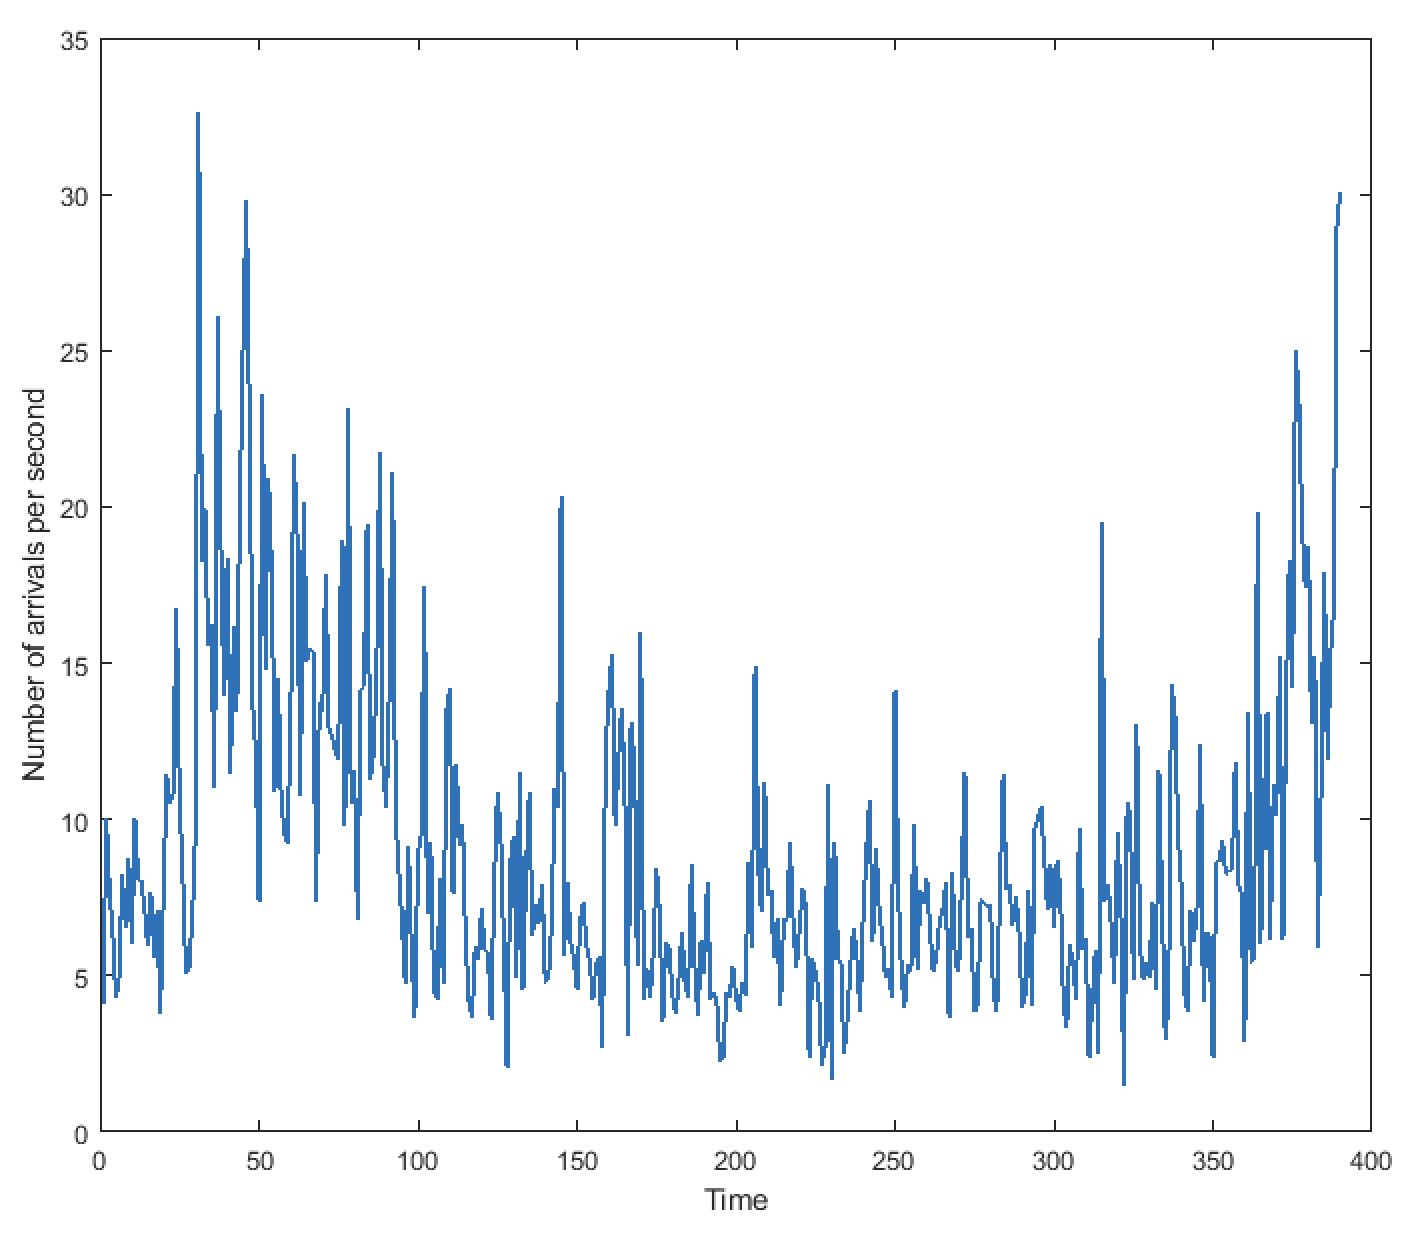
\includegraphics[width=0.75\textwidth]{chapters/chapter_trade_data_models/figures/freqsubmit.png} 
   	\caption{Frequency of Limit Order submission for 09/01/2010 (time in minutes after market opening). \label{fig:freqsubmitarrivals}}
	\end{figure}


This means that if we choose to look at the Limit Order flow with a model that doesn't allow for a varying baseline intensity, we will have to drop these two periods of increased trading activity and keep the data for only the middle portion of 6 hours of the trading day.


We then looked at the data for the central portion of 6 hours of the trading day and found that market orders are just a function of Limit Orders. There were almost 90,000 Limit Orders submitted during that period of the day, compared to the only about 4,000 Market Orders. Similarly, there is an imbalance in the side of the order submission, with around 42,000 Limit Orders submitted on the Sell side compared to the 48,000 submitted on the Buy side (about 18\% more). This side-imbalance is also present in the Market Order submission although not that strongly: 1,882 Market Orders submitted on the Sell side compared to the 2,107 orders submitted on the Buy side (only about 12\% more). 
	\begin{table}
	\centering
	\caption{XOM data for 09/01/2010 \label{tab:xom}}
	\begin{tabular}{llll} 
	& Limit Orders & Market Orders & Total \\ \hline
	Buy & 48,541 & 2,107 & 50,648 \\ 
	Sell & 41,194 & 1,882 & 43,076 \\
	Total & 89,735 & 3,989 & 93,724
	\end{tabular}
	\end{table}
This shows how, on this trading day, most of the ``action'' was occurring on the Buy Side of the book which could mean that the markets were confident in an increase of the price of XOM (in line with the historical performance of the stock for that day).


Our next step was to re-construct the Limit Order book from the order flow so to look at the life of the Limit Orders after their submission. We first looked into how many of the submitted Limit Orders get executed and, when they do, in how many fills. We found Table~\ref{tab:LOexec} that only about 6.5\% of all submitted LOs get at least partially filled with the percentage dropping to only about 6\% for those LO that actually get completely executed. Also, out of the LO that are completely filled nearly 90\% of them is filled in just one execution. This allows us to say that the magnitude of the LOs is comparable to that of the Market Orders, given that nearly all of them require only one Market Order to fill it completely. It is also interesting to note how few of the LOs that are submitted actually get executed. 
	\begin{table}
	\centering
	\caption{LO executions and percentage breakdown by number of fills required \label{tab:LOexec}}
	\begin{tabular}{cccc}
	Number of LO & \% at least partially fill & \% completed in one fill & \% completely fill \\
	89, 735 & 6.57 & 5.35 & 6.15
	\end{tabular}
	\begin{tabular}{ccccccc}
	1 & 2 & 3 & 4 & 5 & 6 & $\geq$ 7 \\ \hline
	87.14 & 10.83 & 1.34 & 0.37 & 0.13 & 0.06 & 0.13
	\end{tabular}
	\end{table}


This means that either very few LO are actually submitted close to the market (hence have a chance to get executed) or that many of them don't stay in the book long enough to get executed. This led us to look into the life-time of the LOs and, more specifically, at their cancellation and execution times. We focused on how long, on average, for an order to be either not filled or partially filled LO stayed in the book before getting cancelled and at how long did it take for a LO to be either filled for the first time or completely filled. Results are given in Table~\ref{tab:meanlo}.
	\begin{table}
	\centering
	\caption{Mean LO cancellation and execution times (in seconds) \label{tab:meanlo}}
	\begin{tabular}{cccc}
	\multicolumn{2}{c}{No Fills} & \multicolumn{2}{c}{Partial Filles} \\ \hline
	Buy Orders & Sell Orders & Buy Orders & Sell Orders \\ \hline
	177.8 & 250.5 & 46.1 & 63.0 \\ \hline
	\multicolumn{2}{c}{First Fill} & \multicolumn{2}{c}{Completion} \\ \hline
	 25.3 & 56.2 & 25.6 & 57.6
	\end{tabular}
	\end{table}

In this particular case, LOs stay in the book for much longer if they are on the sell side than if they are on the buy side. Orders that have never been filled are cancelled after 250 seconds if they are on the sell side compared to 177 seconds if they are on the buy side. Similarly, a partially filled LO on the sell side is cancelled after 63 seconds compared to 46 seconds if it's on the other side of the book. Also, if we look at the time it takes for a LO to be filled for the first time we see that that happens after about 56 seconds on the sell side compared to only 25 seconds on the buy side. Finally, for the LO that do get completely filled, it takes on average 1 minute for that to happen if the order is on the sell side compared to only 25 seconds if the order is on the buy side. This life-time difference for LOs on the two opposite sides of the book is consistent with what we saw earlier in the imbalance of the LO and MO submission. In fact, in this case as well we see how the buy side appears to be the more active side of the book. The shorter execution times for the orders on the buy side could be caused by either more aggressive pricing or by the price movements of the markets while the shorter lifespans and the higher number of orders on that side seem to indicate the use of more active trading strategies. However, there is another interesting observation that can be made. We see that on average a sell LO that is filled for the first time (but that doesn't get completely filled), is cancelled after about 7 seconds, compared to the 20 seconds that it would take had the order been on the buy side. This means that on average it takes three times longer for a partially (and never completely) filled order to be cancelled if it is on the buy side (which is the more active side) that if it is on the sell side (which is the less reactive side). The asymmetry between buy and sell side at the aggregated level has been noted in the literature.


The next step was to observe changes in the behavior of the book when moving further away from the market. We looked into the order submission and cancellation frequencies as a function of distance from the market price. Figure~\ref{fig:canfreq} and Figure~\ref{fig:freqsubmit1} show that most LO are submitted and cancelled at the market (respectively, 40\% and almost 30\%) and that the rates drop sharply with each price level further away from it. This supports the conclusion that the very small percentage of executed LO is not caused by the fact that most LO are submitted far away from the market and hence don't get the chance to get executed. We can also see how approximately 70\% (96\%) of all Limit Orders is placed in the top 5 (20) levels of the book and that 69\% (96\%) of all cancellations also occurs in the top 5 (20) levels. This a first indication of the fact that Level III data offers more information than Level II since with the top 5 levels of the book we were only able to capture around 70\% of all the occurring events. However, this also indicates that there is no need to use all the information provided in Level III data since by looking at only the top 20 levels of the book we are still able to capture nearly all of the occurring events. Both plots show a very similar behavior for the buy and sell side which led us to assume an almost symmetric behavior of the book. This assumption was later tested and confirmed at a 99\% confidence level with a two-sided Kolmogorov-Smirnov Test. 
	\begin{figure}[!ht]
   	\centering
   	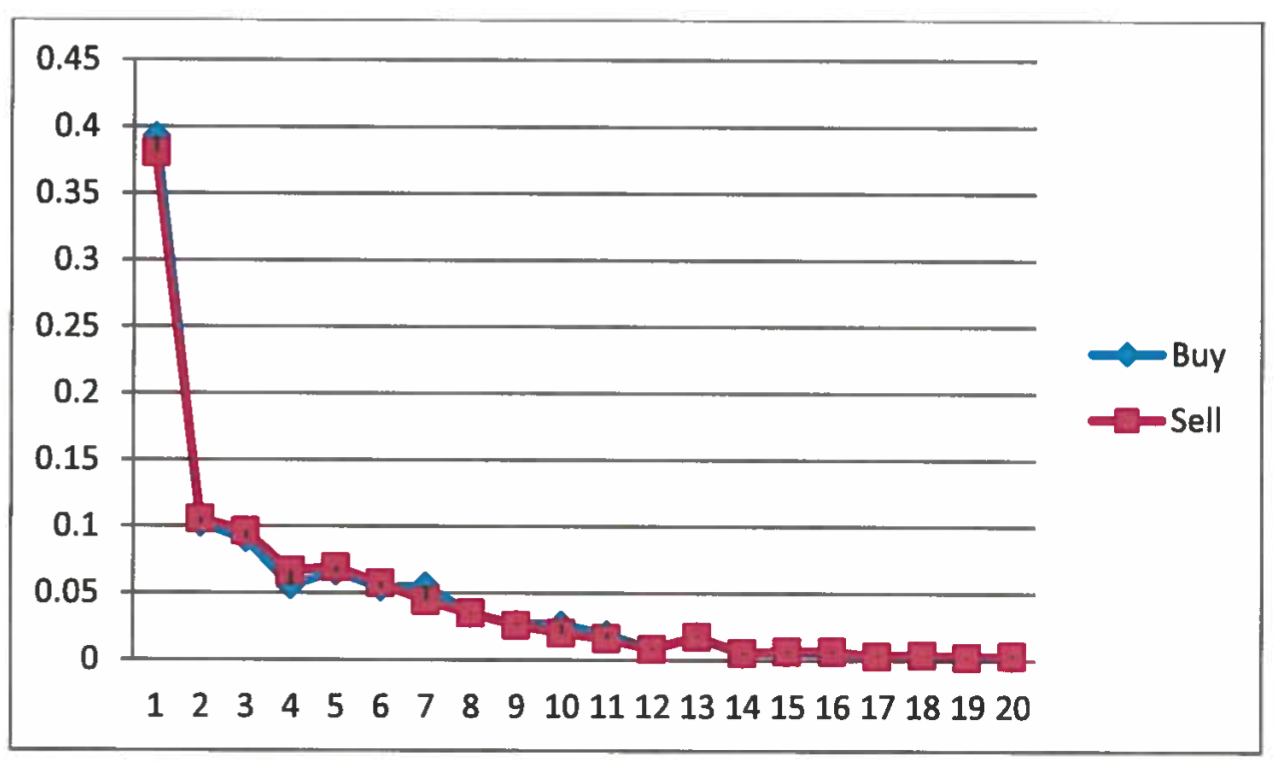
\includegraphics[width=0.75\textwidth]{chapters/chapter_trade_data_models/figures/subfreqnear.png} 
   	\caption{Submission frequencies--Distance near touch price \\ Kolmogorov-Smirnov Test Statistics$=0.61 \to$ fail to reject null at 1\% sig. level \label{fig:subfreqnear}}
	\end{figure}
	\begin{figure}[!ht]
   	\centering
   	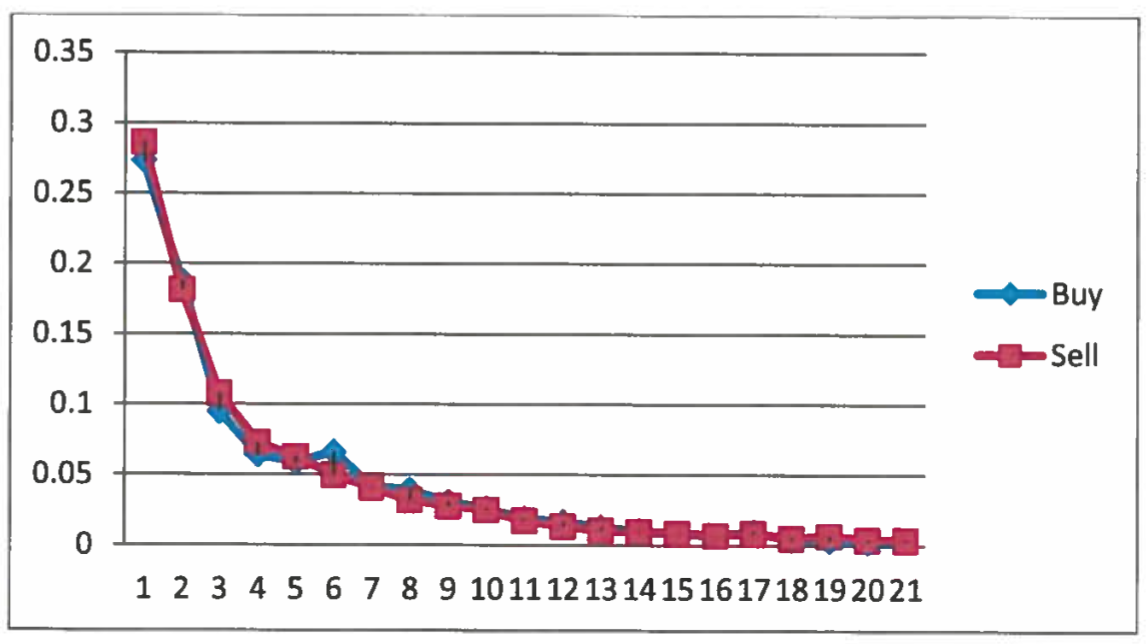
\includegraphics[width=0.75\textwidth]{chapters/chapter_trade_data_models/figures/canfreqnear.png} 
   	\caption{Cancellation Frequencies--Distance from near touch price \\ Kolmogorov-Smirnov Test Statistic$=0.83\to$ fail to reject null at 1\% sig. level \label{fig:canfreqnear}}
	\end{figure}


Better understanding what happens to the LOs once they enter the book is key in developing a more accurate way of choosing when to submit a LO or a MO. For this reason we also looked at the cancellation frequencies as a function of position in the queue and we found that (Figure~\ref{fig:canfreq}) most of the cancellations occur when the LO are in 4th or 5th position in the queue. In this case as well, we carried out a test of the assumption of a symmetric behavior of the book which confirmed previous similar findings. However, it would be more interesting to look at the cancellation frequencies as a function of overall distance from the market (as a measure of distance from possible execution). 
	\begin{figure}[!ht]
   	\centering
   	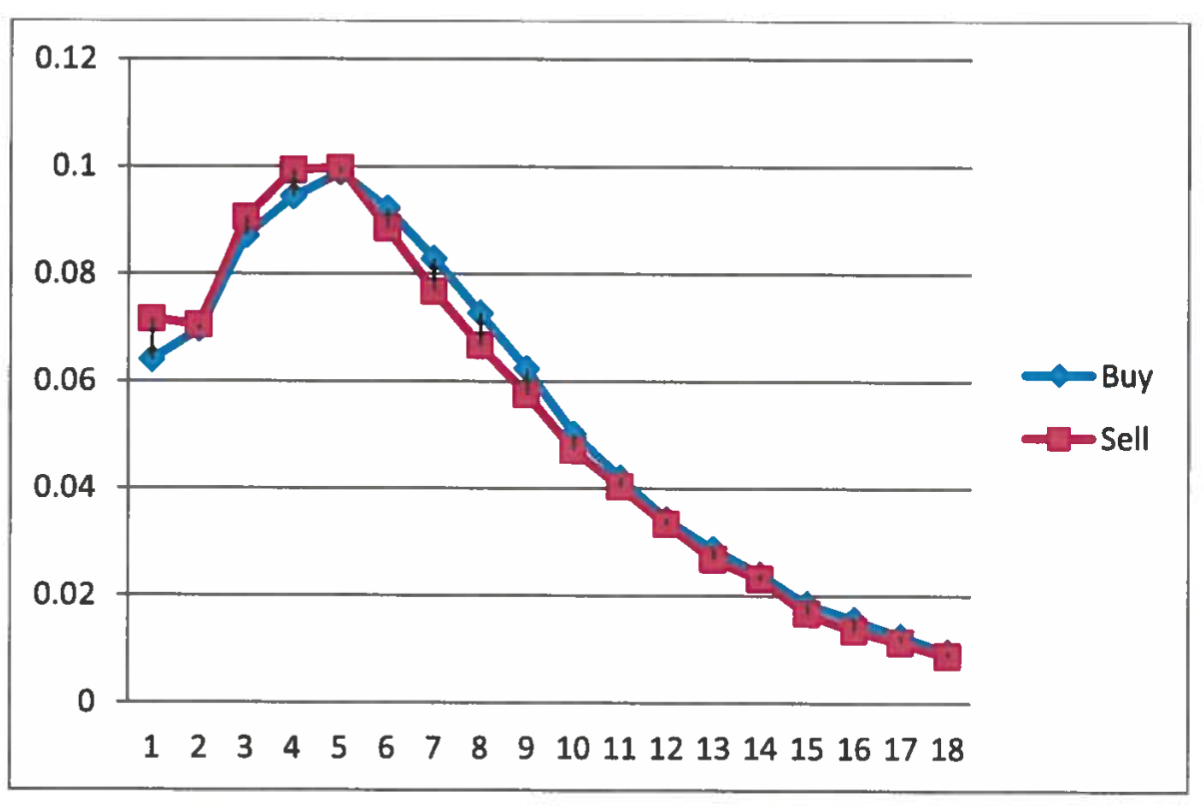
\includegraphics[width=0.75\textwidth]{chapters/chapter_trade_data_models/figures/canfreq.png} 
   	\caption{Cancellation Frequencies---position in queue. \label{fig:canfreq}}
	\end{figure}


With two more trading days (3rd and 9th of September 2013) data available, we are able to study the robustness of the above results. The submission and cancellation frequencies as a function of relative price which were symmetric for the 1st of September were not symmetric anymore on the 3rd of September. In this trading day, Figure~\ref{fig:freqsubmit1}, the peak of activity on the buy side occurred 12 price levels away from the market. This seems to suggest that on the 3rd of September the markets were betting that the price of XOM would drop in the foreseeable future, possibly reacting to some new event. A closer investigation of that time period revealed in the previous days the announcement by Exxon Mobil of the plan of closing a refinery which then led to a drop in the price shortly after 09/03/2010.
	\begin{figure}[!ht]
   	\centering
   	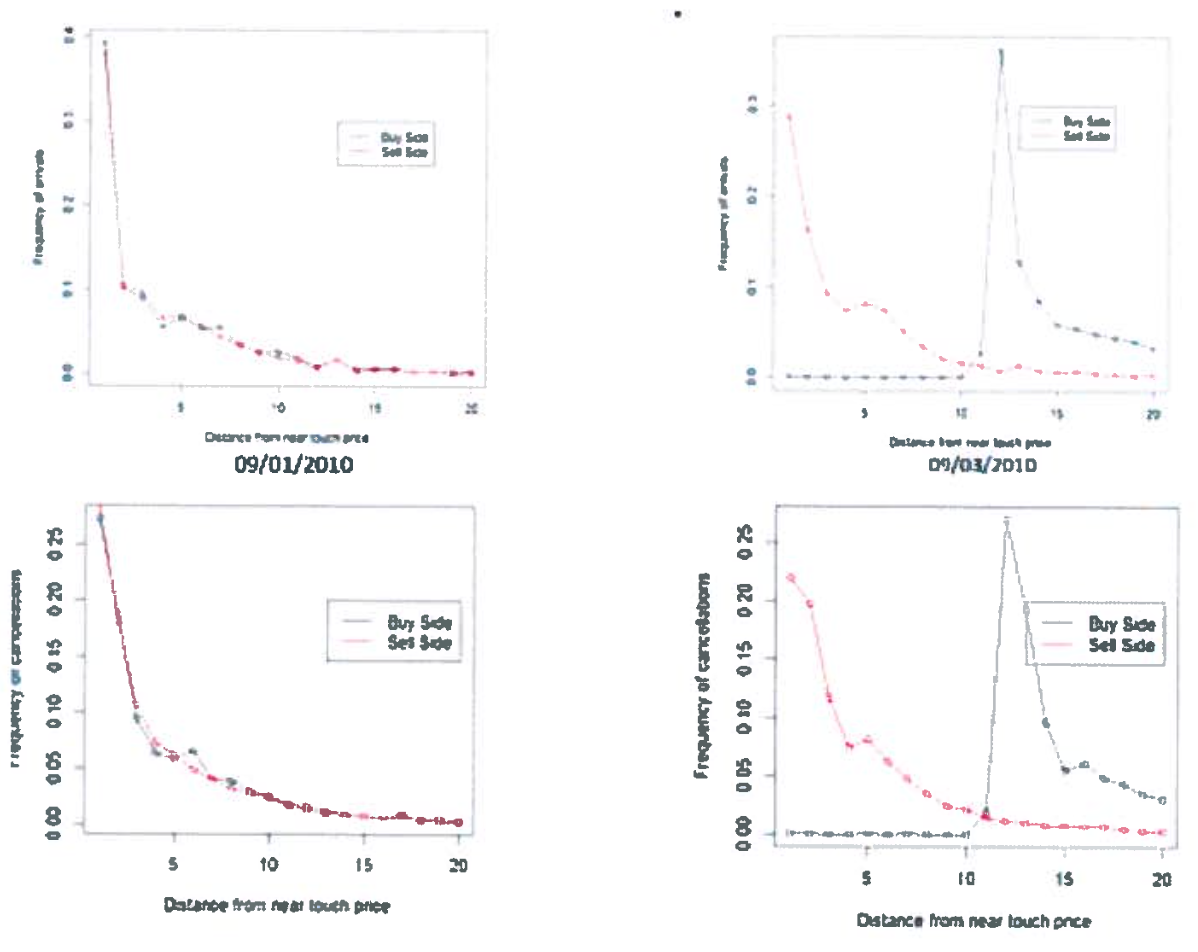
\includegraphics[width=0.75\textwidth]{chapters/chapter_trade_data_models/figures/losubcanfreq.png} 
   	\caption{LO submission and cancellation frequencies. \label{fig:losubcanfreq}}
	\end{figure}


A second interesting difference was in the amount of volume on the two sides of the book (Figure~\ref{fig:losubcanfreq}). Across the 3 days there was a significant volume imbalance with considerably more volume on the sell side than on the buy side but the amount of imbalance between the two sides changes significantly across the three days. Overall there is no explanation as to why there would be such a strong volume imbalance in favor of the sell side other than some kind of temporary anomaly. These findings seem to point out the fact that the shape and behavior of the LOB change dramatically across different days and that, in order to capture some kind of more general/average behavior of the book, many more days of data are required. 
	\begin{figure}[!ht]
   	\centering
   	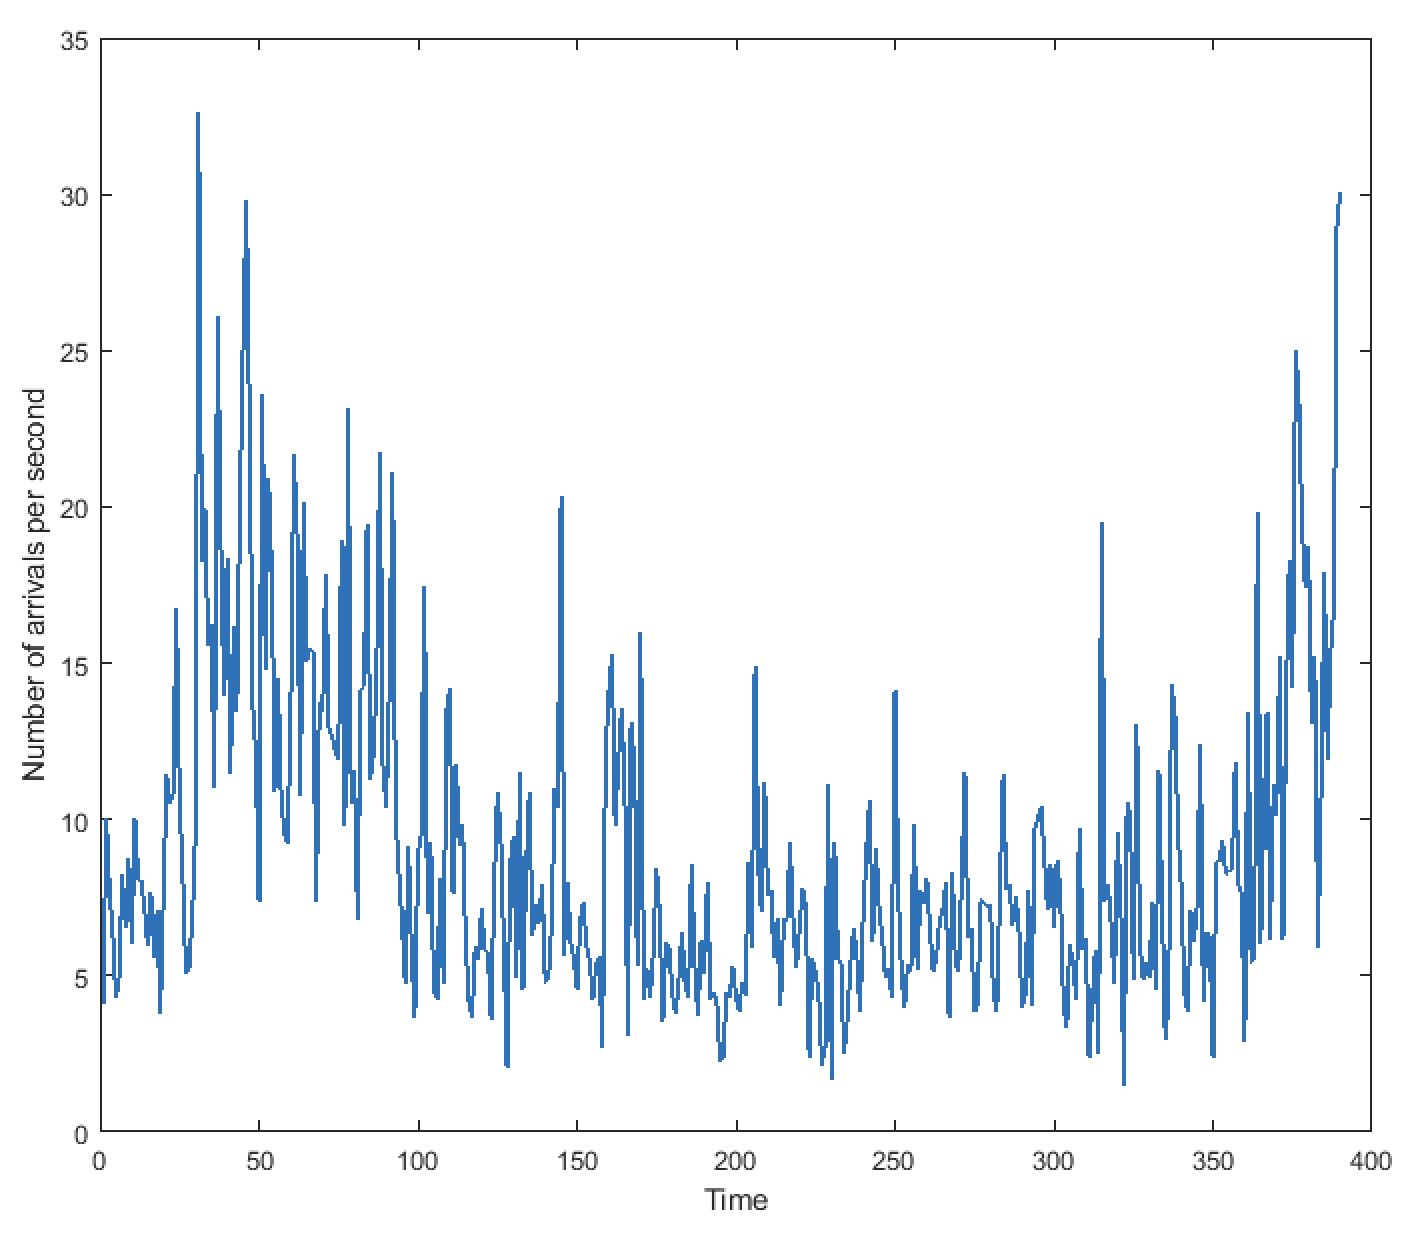
\includegraphics[width=0.75\textwidth]{chapters/chapter_trade_data_models/figures/freqsubmit.png} 
   	\caption{Frequency of Limit Order submission for 09/01/2010 (time in minutes after market opening). \label{fig:freqsubmit1}}
	\end{figure}
	\begin{figure}
	\centering
	\begin{subfigure}
	  \centering
	  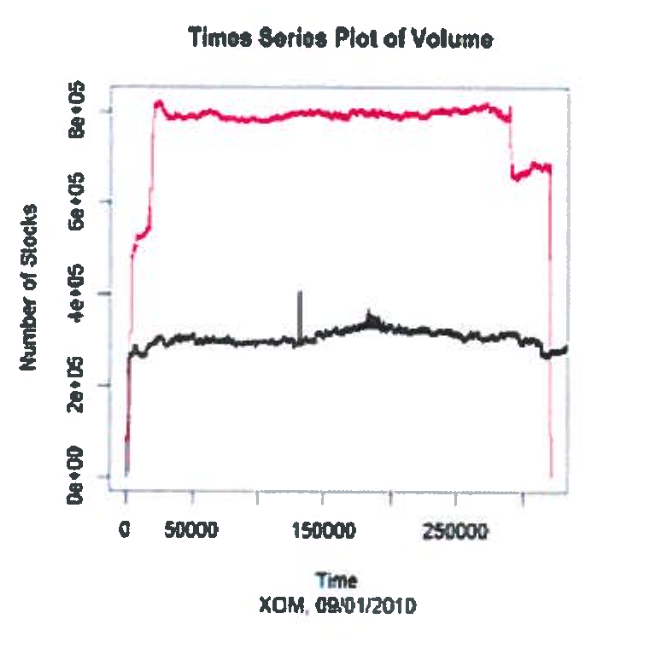
\includegraphics[width=.4\linewidth]{chapters/chapter_trade_data_models/figures/timevol1.png}
	\end{subfigure}%
	\begin{subfigure}
	  \centering
	  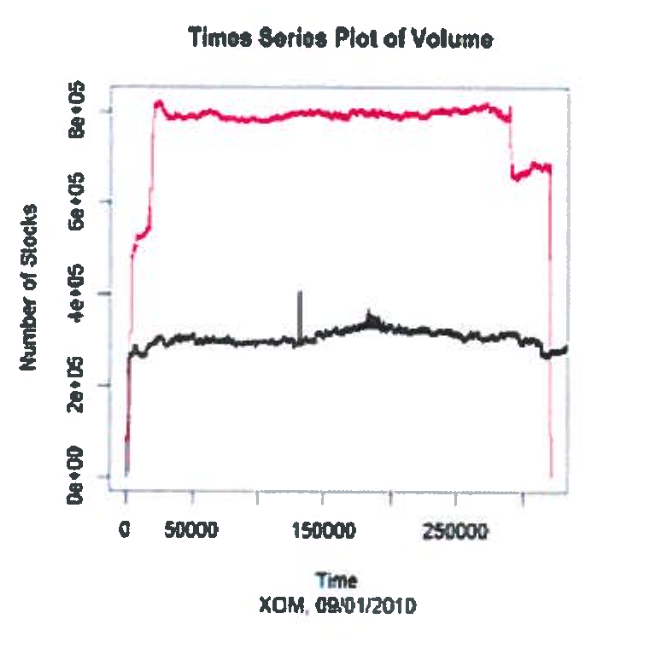
\includegraphics[width=.4\linewidth]{chapters/chapter_trade_data_models/figures/timevol1.png}
	\end{subfigure}
	\caption{Frequency of Limit Order submission for 09/01/2010 (time in minutes after market opening). \label{fig:freqsubmit2}}
	\end{figure}


\subsubsection{One-Dimensional Models}


We started by building a one dimensional model for the Limit Orders submitted on the buy side and one for those submitted on the sell side. Similarly, we build a one dimensional model for the Market Orders submitted on each side of the book. In the one dimensional case, the intensity function driving the Hawkes process is of the form
	\begin{equation}\label{eqn:lambda6}
	\lambda(t)= \lambda_0 + \alpha \sum_{t_i<t} e^{-\beta(t-t_i)}
	\end{equation}
with $\lambda_0$ indicating the baseline intensity, $\alpha$ indicating the jump in the intensity after the occurrence of an event and $\beta$ indicating the rate of exponential decay of the intensity after the occurrence of an event.


Table~\ref{tab:limmodbuy} and Table~\ref{tab:limmodsell} show the results of the MLE estimation of the parameters of the one dimensional models for the Limit Orders on the two sides of the book. The difference in the values of the estimates of the parameters for the two sides of the book (strongest on the 9th and weakest on the 1st of September) indicates that there is a level of asymmetry between these two sides. Also, even though the magnitude of the values of the parameters is the same for all three days (on each side of the book) there is still some variation between them, especially when we look at the model for the buy side. This seems to suggest that the behavior of the book can change considerably from day to day and that a considerable amount of data might be necessary in order to capture some kind of general behavior. 
	\begin{table}
	\centering
	\caption{1-D Limit Order Model (buy side) \label{tab:limmodbuy}}
	\begin{tabular}{c|ccc} 
		& $\lambda$ & $\alpha$  & $\beta$ \\ \hline
	09/01/2010 & 0.008108431 & 1.421767060 & 1.435094466 \\
	09/03/2010 & 0.006127003 & 1.290012415 & 1.299564704 \\
	09/09/2010 & 0.002341542 & 1.023410145 & 1.026757239
	\end{tabular}
	\end{table}
	\begin{table}
	\centering
	\caption{1-D Limit Order Model (sell side) \label{tab:limmodsell}}
	\begin{tabular}{c|ccc} 
		& $\lambda$ & $\alpha$ & $\beta$ \\
	09/01/2010 & 0.002055786 & 1.071071139 & 1.073989940 \\
	09/03/2010 & 0.002342963 & 0.983678355 & 0.986999404 \\
	09/09/2010 & 0.006123845 & 0.946420813 & 0.955774394
	\end{tabular}
	\end{table}


One of the advantages of having chosen an exponential decay for the intensity function of the process, becomes apparent when we analyze the meaning of these parameters. Using a well-known property of exponentially distributed variables, we can tell the half-life of the excitation effect caused by the occurrence of an event. In the specific, in our one-dimensional models we find that, on average, half of the excitation effect caused by the occurrence of an event is dissipated after about 0.7 seconds ($\frac{\ln 2}{\beta} \approx$ half-life). Also, the small estimated values for $\alpha$ indicate that the occurrence of an event has a very small impact on the likelihood of another event occurring. This seems to suggest that there is a weak self-excitation effect in the LO process when modeling it with a one-dimensional model. 


We then build, in a similar fashion, the two one-dimensional models for the flow of buy and sell Market Orders for all three days and obtained the following parameter estimation: 
	\begin{table}[!ht]
	\centering
	\caption{1-D Market Order Model (buy side) \label{tab:marketorderbuy}}
	\begin{tabular}{c|ccc} 
		& $\lambda$ & $\alpha$ & $\beta$ \\ \hline
	09/01/2010 & 0.0238743 & 7.3187478 & 19.8477514 \\
	09/03/2010 & 0.01450873 & 3.38168999 & 7.70581048 \\
	09/09/2010 & 0.0267254 & 4.8818834 & 13.5427254
	\end{tabular}
	\end{table}
	\begin{table}[!ht]
	\centering
	\caption{1-D Market Order Model (sell side) \label{fig:marketordersell}}
	\begin{tabular}{c|ccc} 
		& $\lambda$ & $\alpha$  & $\beta$ \\ \hline
	09/01/2010 & 0.02083999 & 9.38842281 & 24.55777564 \\
	09/03/2010 & 0.01616096 & 6.64370599 & 16.68090519 \\
	09/09/2010 & 0.0239992 & 8.2180945 & 25.0115980
	\end{tabular}
	\end{table}
The first thing that is obvious is the asymmetry between the buy and the sell sides. Nevertheless, for the Market Orders they asymmetry appears to be much more significant that it was for the Limit Orders, given the much bigger differences in the values of the estimated parameters. Also, for Market Orders we see that the occurrence of each event seems to have a much stronger impact on the likelihood of occurrence of future events than it was the case for Limit Orders. In fact, the values of $\alpha$ in Table~\ref{tab:marketorderbuy} and Table~\ref{fig:marketordersell} are considerably higher than those we saw in Table~\ref{tab:limmodbuy} and Table~\ref{tab:limmodsell}. Similarly, the values of $\beta$ are also much larger in the Market Order models than they were in the Limit Order models which means that the half-life of the excitation effect is much shorter for Market Orders (0.03 seconds vs. 0.7 seconds) than for Limit Orders. These differences in the results of the estimations are not that surprising if we consider what we saw in Table~\ref{tab:xom} for order submissions. Market Orders are submitted in much fewer numbers than Limit Orders which explains why even though the occurrence, such self-excitation has a very short lifetime. The significant increase in the chances of another Market Order occurring given that one has just occurred (even through for a very short time), might seem contradicting the fact that very few Market Orders actually occur. However, what can be inferred is that Market Orders depend strongly from the occurrence of other Market Orders and that they tend to cluster around submissions. 


\subsubsection{An extension}


An important limitation of this basic Hawkes Process model is that each event has the same impact on the intensity function. This implies that each event carries the same amount of information in the process. However, it is easy to imagine that a large LO would carry much more information about future price changes than a small one and this should be accounted for in the model. We include order size in the intensity function by scaling the size of the jump $\alpha$ in the value of the intensity by the ratio $\frac{w_i}{\overline{w}_l}$, where $w_i$ is the size of the LO and $\overline{w}_l$ is the average LO size up to that point. The intensity function for this ``extended'' one-dimensional model becomes
	\[
	\lambda(t)= \lambda_0 + \alpha \sum_{t_i<t} \dfrac{w_i}{\overline{w}_l} e^{-\beta(t-t_i)}
	\]
We then compared the performance of this ``size-adjusted'' model with the ``basic'' one by using the before mentioned \emph{Multivariate Random Time Chance} Theorem and looking at the Q-Q plot of the compensators for the two models. Figure~\ref{fig:lobuysideadj} and Figure~\ref{fig:losellsideadj} show how in both case (buy and sell Limit Orders) adjusting for size doesn't improve the fit of the model. This result is somewhat counter-intuitive given that more than 70\% of all Limit Orders are of size 100 shares and that this should imply that any deviation from this size explanation is that trading strategies are successful in concealing the true intension of the traders and that there is no significant information left in the size of the LO once that the strategies are implemented and the orders are submitted. 
	\begin{figure}[!ht]
   	\centering
   	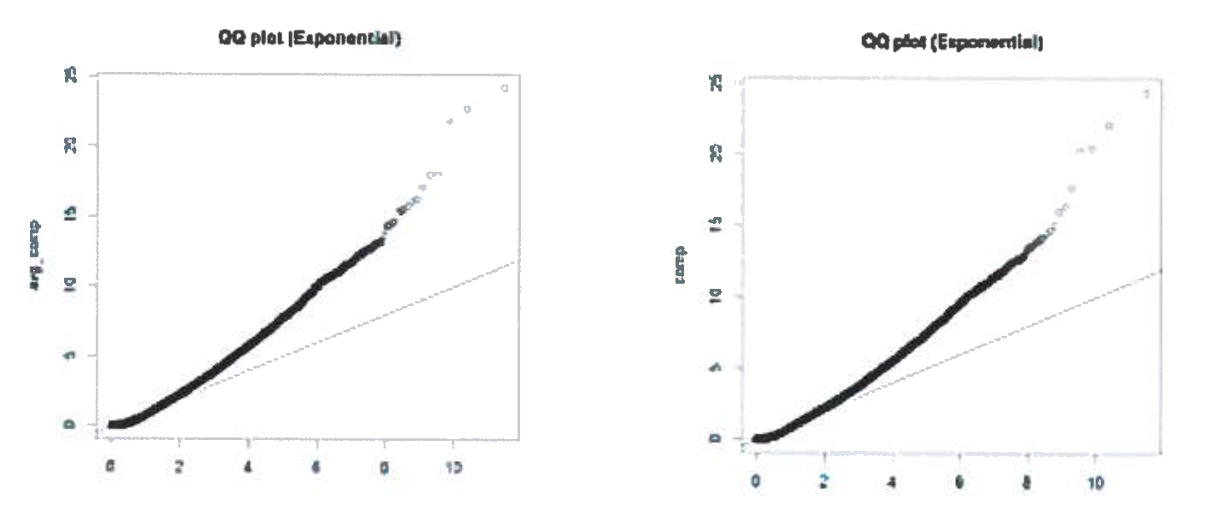
\includegraphics[width=0.75\textwidth]{chapters/chapter_trade_data_models/figures/lobuysideadj.png} 
   	\caption{LO--buy side with size adjustment and without. \label{fig:lobuysideadj}}
	\end{figure}
	\begin{figure}[!ht]
   	\centering
   	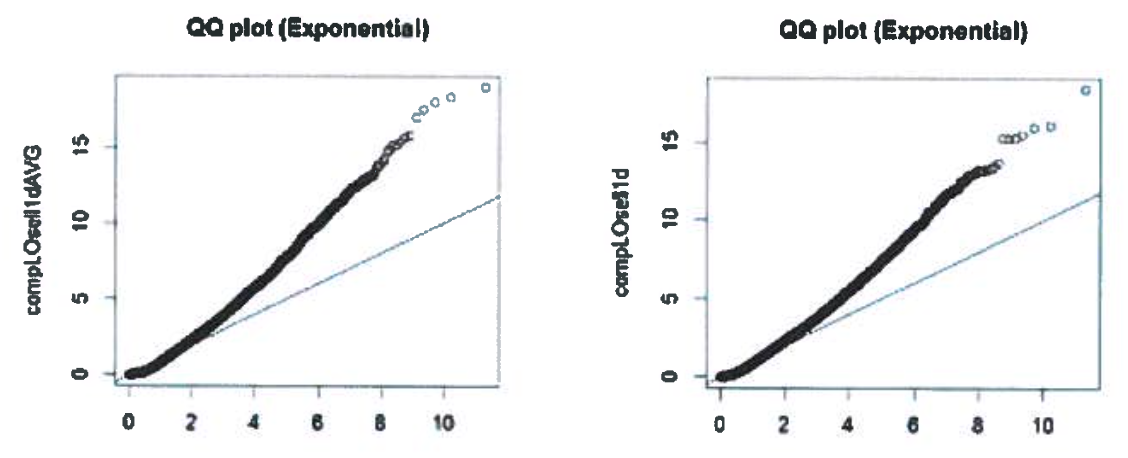
\includegraphics[width=0.75\textwidth]{chapters/chapter_trade_data_models/figures/losellsideadj.png} 
   	\caption{LO--sell side with size adjustment and without. \label{fig:losellsideadj}}
	\end{figure}


\subsubsection{Two-Dimensional models}


Our next step was to build two-dimensional models that would simultaneously model the buy and sell sides of the book and with two separate (yet interacting) intensity functions. The intensity functions for this kind of model become
	\[
	\begin{split}
	\lambda^B(t)&= \lambda_0^B + \int_0^t \alpha^{BB} e^{-\beta^{BB}(t-u)} \;dN_u^B + \int_0^t \alpha^{BB} e^{-\beta^{BS}(t-u)} \;dN_u^S \\
	\lambda^S(t)&= \lambda_0^S + \int_0^t \alpha^{SB} e^{-\beta^{SB}(t-u)} \; dN_u^B + \int_0^t \alpha^{SS} e^{-\beta^{SS}(t-u)} \;dN_i^S
	\end{split}
	\]
and we have 5 parameters for each dimension of the model for a total of 10 parameters across the two dimensions (buy and sell). The two additional parameters in each dimension account for the cross-excitation effect between the two dimensions. In our case, $\alpha^{BS}$ tells us the increase in the likeliness of a LO occurring on the buy side after the occurrence of a LO on the sell side, while $\beta^{BS}$ tells us the rate of decay of the buy side intensity after the occurrence of a LO on the sell side (and vice-versa for $\alpha^{SB}$ and $\beta^{SB}$). We then used MLE to estimate the parameters of the model and we can make several remarks about the results (Table~\ref{tab:2dimlomodel}).
	\begin{table}
	\centering
	\caption{2-Dimensional LO model \label{tab:2dimlomodel}}
	\begin{tabular}{lllll}  
	$\lambda^B=2.480 \cdot 10^{-5}$ & $\alpha^{BB}=14.386$ & $\beta^{BB}=31.517$ & $\alpha^{BS}=0.303$ & $\beta^{BS}=0.464$ \\ \hline
	$\lambda^S=2.677 \cdot 10^{-5}$ & $\lambda^{SS}=15.657$ & $\beta^{SS}=37.299$ & $\alpha^{SB}=0.149$ & $\beta^{SB}=0.312$ \\ 
	\end{tabular}
	\end{table}
	
	
There appears to be some asymmetry in the cross-excitation effects with the occurrence of an event on the sell side having a stronger impact on the likeliness of occurrence of an event on the buy side rather than the other way round ($\alpha^{BS}>\alpha^{SB}$). On the other hand though, since $\beta^{BS}<\beta^{SB}$, the effect on the sell side of an occurrence on the buy side is more persistent than that of an event on the buy side on the sell side (2.22 seconds vs. 1.49 seconds).
	\begin{figure}[!ht]
   	\centering
   	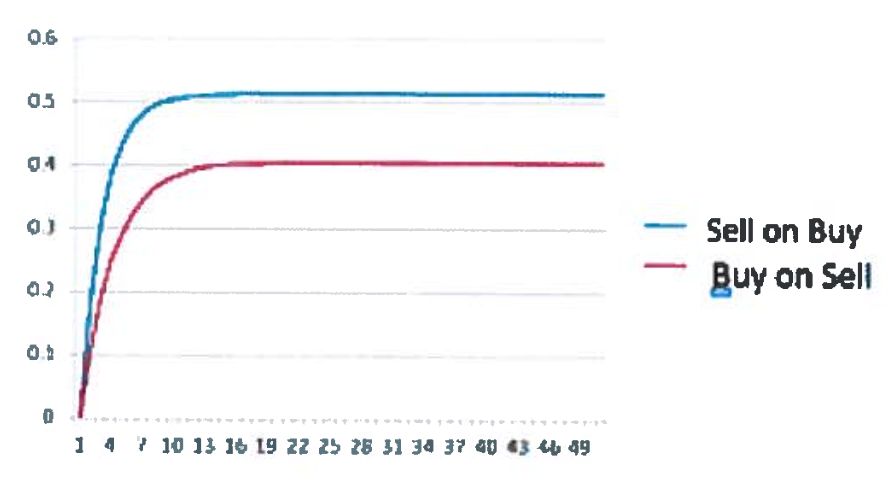
\includegraphics[width=0.75\textwidth]{chapters/chapter_trade_data_models/figures/asymcross.png} 
   	\caption{Asymmetry in cross-excitation effect. \label{fig:asymcross}}
	\end{figure}
The self-excitation components of the model are rather similar for both dimensions and it is interesting to point out the very short persistence of the self-excitation effect in both cases (about 0.02 seconds).


In order to evaluate whether the two key features of a model based on Hawkes processes (path dependency of the order flow and the possibility of modeling the relation between the various dimensions) are really helpful in improving the performance of the model, we decided to compare the performance of our model to that of a bi-dimensional model based on two independent Poisson Processes (which by definition of Poisson process cannot account for any dependency in the order flow and by construction assume independence between the two dimensions). The results proved to be very encouraging with a remarkably better fit to the empirical data for the Hawkes Process based model (Figure~\ref{fig:4hawkes6}).
	\begin{figure}[!ht]
   	\centering
   	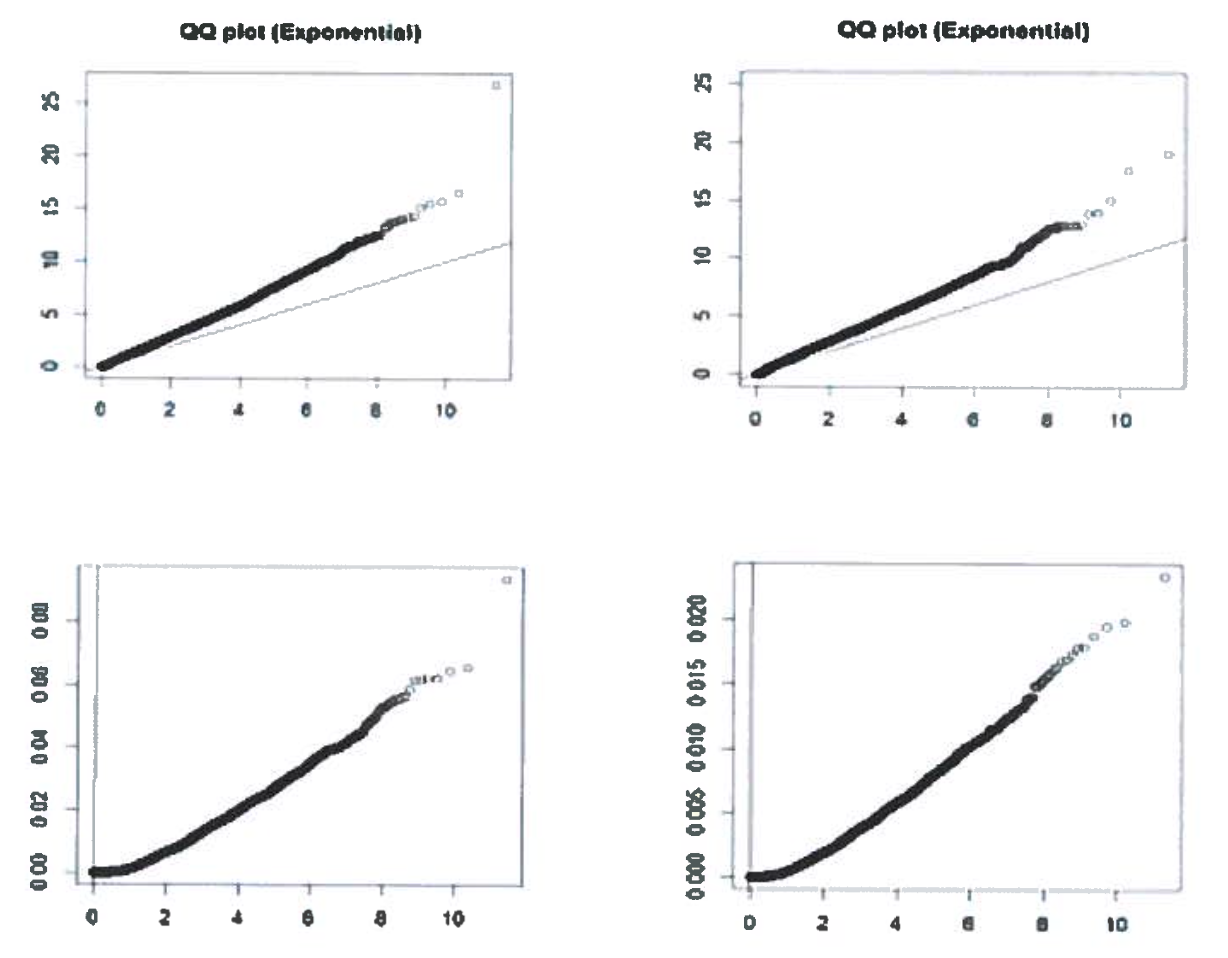
\includegraphics[width=0.75\textwidth]{chapters/chapter_trade_data_models/figures/4hawkes6.png} 
   	\caption{Top--Fit of Hawkes Process (buy \& sell); Bottom--Fit of Poisson Process (buy \& sell). \label{fig:4hawkes6}}
	\end{figure}


Following a similar procedure, we build a bi-dimensional model for the Market Orders and performed MLE to estimate the parameters. The results (Table~\ref{tab:2dimmomod}) showed very weak and symmetric cross-excitation between the dimensions which, however, turns out to be very persistent (141 seconds for the half-life of the effect of buy on sell and 215 seconds for that of sell on buy). The self-excitation effect is comparable across the two dimensions and is also very short lived (with a half-life of about 0.02 seconds).
	\begin{table}
	\centering
	\caption{2-Dimensional MO model \label{tab:2dimmomod}}
	\begin{tabular}{lllll}  
	$\lambda^B=2.701 \cdot 10^{-5}$ & $\alpha^{BB}=11.793$ & $\beta^{BB}=36.153$ & $\alpha^{BS}=0.0037$ & $\beta^{BS}=0.0049$ \\
	$\lambda^S=3.451 \cdot 10^{-5}$ & $\alpha^{SS}=12.454$ & $\beta^{SS}=35.063$ & $\alpha^{SB}=0.0017$ & $\beta^{SB}=0.0032$
	\end{tabular}
	\end{table}
	

Finally, we compared the performance of our model to that of the bi-dimensional Poisson Process. Similarly to the LO case, the model at hand significantly outperforms the Poisson Process one for both dimensions. 
	\begin{figure}[!ht]
   	\centering
   	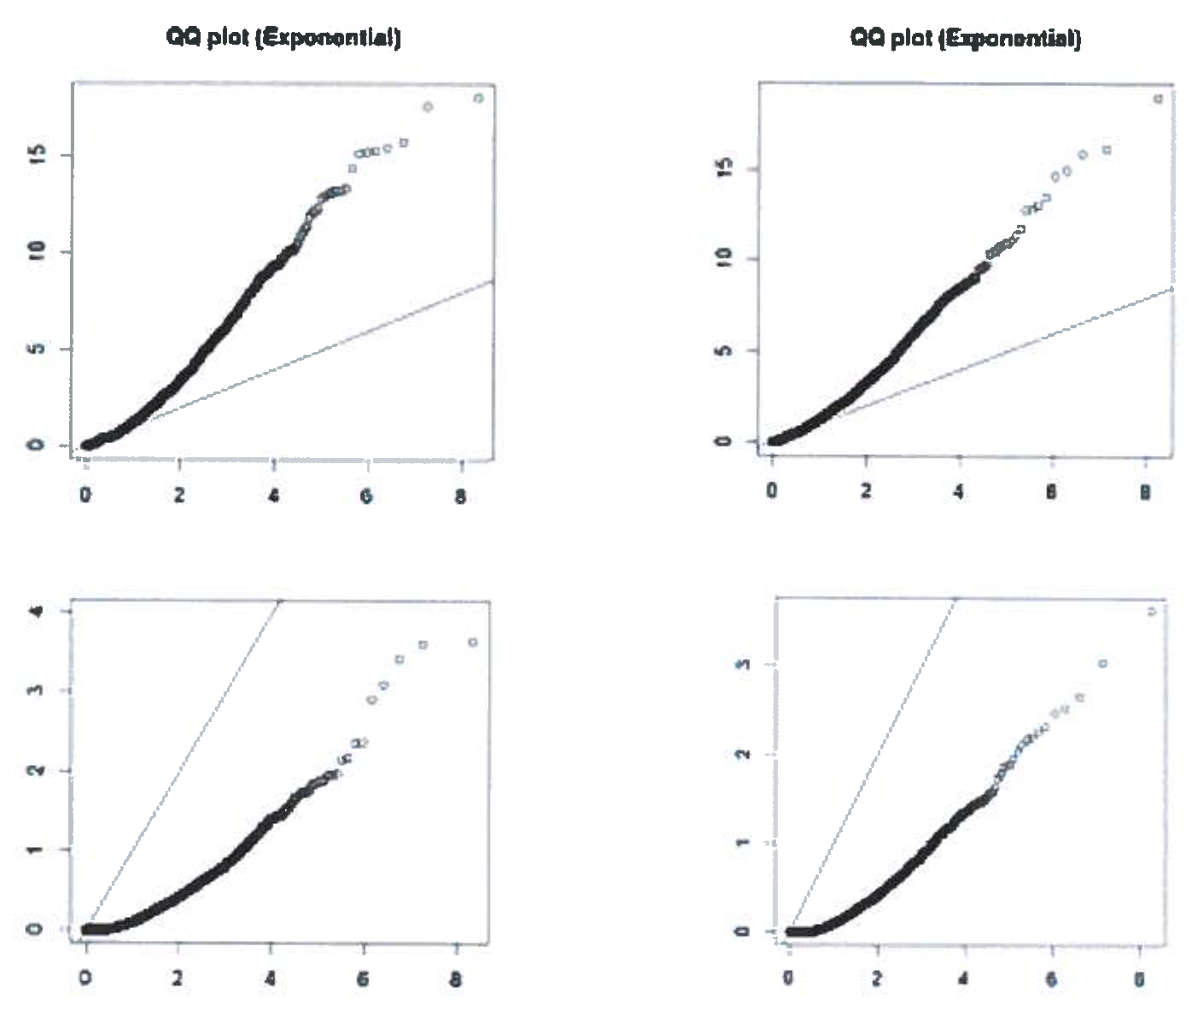
\includegraphics[width=0.75\textwidth]{chapters/chapter_trade_data_models/figures/4fig.png} 
   	\caption{Top--Fit of Hawkes Process (buy \& sell); Bottom--Fit of Poisson Process (buy \& sell). \label{fig:4fig6}}
	\end{figure}


\subsubsection{Limitations and findings}


There are some important considerations to be made based on our analysis. The first issue is related to the cleaning of the data that was necessary in order to adapt it to our needs. In fact, Hawkes processes are ``simple'' processes which means that they don't allow for more events to occur simultaneously. Unfortunately, in the INET data it is quite common to encounter clusters of 10/20 events reported with the same timestamp. This is typical of high frequency data due to the approximation with which events are often reported and to the obvious limitation of the chosen time scale (e.g., milliseconds). In our case we decided to keep only the first event of each cluster, dropping all the others. A possible alternative used in the literature is to simply uniformly distribute the events from the clusters across the time interval given by the occurrence of the cluster and that of the next event. However, this approach could introduce bias in the parameter estimation phase. In fact, the clustering of events by itself is of interest.


Also, an important limitation of the bi-dimensional Hawkes Process model is that it is very computationally intense. Evaluating the 5 parameters for one of the two intensity function using data from only one trading day took almost 48 hours. It becomes clear that in order to evaluate the parameters of a model using data for a longer time period of if evaluating the parameters for a model with higher dimension (hence with more parameters) will require considerably more computational power. 

\subsection{Models for Hidden Liquidity}
TODO
\section{Supplements and Problems} 
TODO
